\mychapter{Results}{Results}{}\label{chap:results}

\section{Overview}
\label{sec:results_overview}

% Throughout this chapter, the best value in every column of a table is shown in bold.


\section{Experiment 1: Mixed-Facility Baseline}
\label{sec:results_mixed}

\subsection{Clarifiers}
\label{sec:results_mixed_clarifier}

\subsubsection{Comparison Table}

\begin{table}[htbp]
\centering
\caption{Clarifier test results of every architecture on the stratified 70/20/10 split (Experiment~1). Macro-averaged scores give every class the same weight. The best value in every column is shown in bold.}
\label{tab:res_mixed_clarifier}
\setlength{\tabcolsep}{4pt}
\begin{tabular}{lrrrrr}
\toprule
\textbf{Architecture} & \textbf{Accuracy} & \textbf{Mean AUC} & \textbf{\makecell[r]{Macro\\precision}} & \textbf{\makecell[r]{Macro\\recall}} & \textbf{\makecell[r]{Macro\\F1}} \\
\midrule
ResNet-18 & 0.854 & 0.961 & 0.855 & 0.876 & 0.864 \\
EfficientNet-B0 & 0.864 & 0.970 & 0.859 & 0.879 & 0.867 \\
DenseNet-121 & 0.882 & \textbf{0.975} & 0.891 & 0.870 & 0.880 \\
ResNet-50 & 0.836 & 0.968 & 0.812 & 0.837 & 0.821 \\
ConvNeXt-Tiny & \textbf{0.889} & \textbf{0.975} & \textbf{0.894} & \textbf{0.899} & \textbf{0.895} \\
Inception-v3 & 0.868 & 0.968 & 0.855 & 0.875 & 0.864 \\
AlexNet & 0.761 & 0.924 & 0.781 & 0.808 & 0.790 \\
\bottomrule
\end{tabular}
\end{table}

\subsubsection{Accuracy and AUC}

\begin{figure}[htbp]
    \centering
    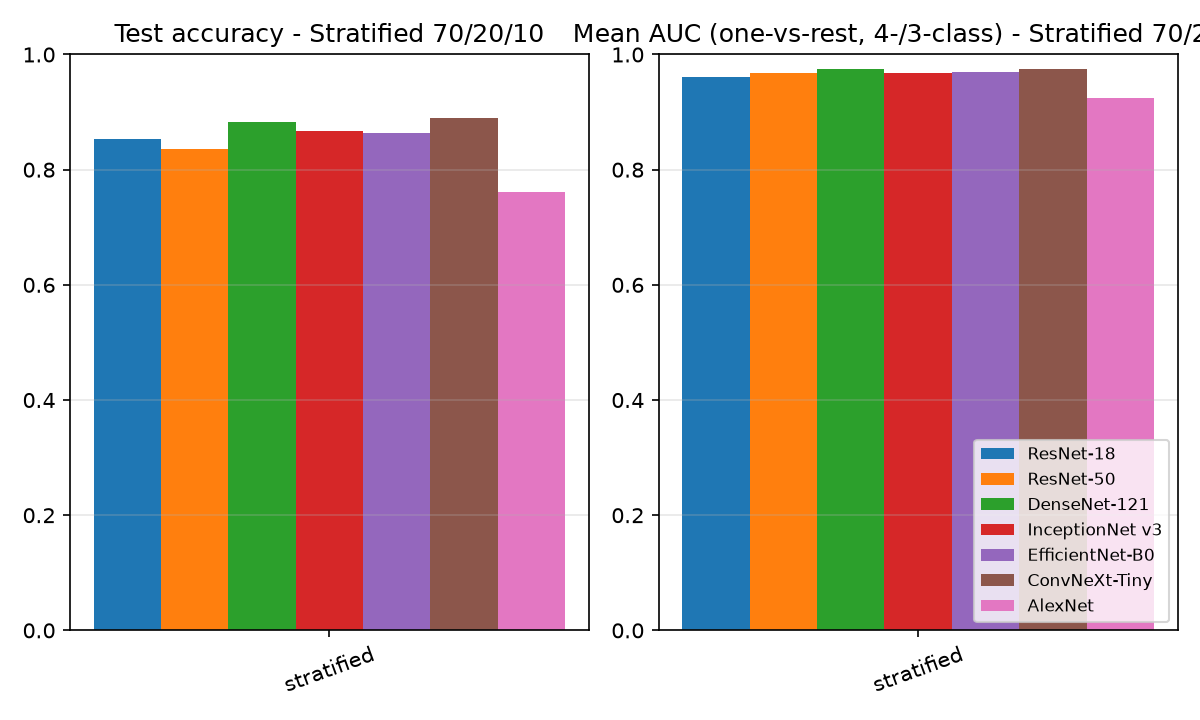
\includegraphics[width=0.75\textwidth]{figures/results/clarifier_stratified_accuracy_auc_bars.png}
    \caption{Test accuracy and mean one-vs-rest AUC of every clarifier architecture on the stratified split (Experiment~1).}
    \label{fig:res_mixed_clarifier_bars}
\end{figure}

\subsubsection{Per-Class Precision, Recall and F1}

\begin{table}[htbp]
\centering
\footnotesize
\setlength{\tabcolsep}{3pt}
\caption{Per-class precision (P), recall (R) and F1 score of every clarifier architecture on the stratified split (Experiment~1).}
\label{tab:res_mixed_clarifier_perclass}
\resizebox{\textwidth}{!}{%
\begin{tabular}{l rrr rrr rrr rrr}
\toprule
& \multicolumn{3}{c}{\textbf{Dysfunctional}} & \multicolumn{3}{c}{\textbf{Empty}} & \multicolumn{3}{c}{\textbf{Functional}} & \multicolumn{3}{c}{\textbf{Scum}} \\
\cmidrule(lr){2-4} \cmidrule(lr){5-7} \cmidrule(lr){8-10} \cmidrule(lr){11-13}
\textbf{Architecture} & P & R & F1 & P & R & F1 & P & R & F1 & P & R & F1 \\
\midrule
ResNet-18 & 0.895 & 0.919 & 0.907 & 0.826 & \textbf{0.905} & 0.864 & 0.826 & 0.896 & 0.860 & 0.875 & 0.784 & 0.827 \\
EfficientNet-B0 & 0.868 & 0.892 & 0.880 & 0.826 & \textbf{0.905} & 0.864 & 0.838 & 0.925 & 0.879 & 0.902 & 0.793 & 0.844 \\
DenseNet-121 & 0.912 & 0.838 & 0.873 & \textbf{0.900} & 0.857 & 0.878 & \textbf{0.882} & 0.915 & 0.898 & 0.871 & \textbf{0.871} & \textbf{0.871} \\
ResNet-50 & 0.882 & 0.811 & 0.845 & 0.667 & 0.857 & 0.750 & 0.839 & 0.887 & 0.862 & 0.860 & 0.793 & 0.825 \\
ConvNeXt-Tiny & \textbf{0.944} & 0.919 & \textbf{0.932} & 0.864 & \textbf{0.905} & \textbf{0.884} & 0.856 & \textbf{0.953} & \textbf{0.902} & \textbf{0.913} & 0.819 & 0.864 \\
Inception-v3 & 0.850 & 0.919 & 0.883 & 0.818 & 0.857 & 0.837 & 0.866 & 0.915 & 0.890 & 0.887 & 0.810 & 0.847 \\
AlexNet & 0.857 & \textbf{0.973} & 0.911 & 0.773 & 0.810 & 0.791 & 0.707 & 0.821 & 0.760 & 0.785 & 0.629 & 0.699 \\
\bottomrule
\end{tabular}}
\end{table}

\subsection{Aerobic Zones}
\label{sec:results_mixed_aerobic}

\subsubsection{Comparison Table}

\begin{table}[htbp]
\centering
\caption{Aerobic zone test results of every architecture on the stratified 70/20/10 split (Experiment~1).}
\label{tab:res_mixed_aerobic}
\setlength{\tabcolsep}{4pt}
\begin{tabular}{lrrrrr}
\toprule
\textbf{Architecture} & \textbf{Accuracy} & \textbf{Mean AUC} & \textbf{\makecell[r]{Macro\\precision}} & \textbf{\makecell[r]{Macro\\recall}} & \textbf{\makecell[r]{Macro\\F1}} \\
\midrule
ResNet-18 & 0.768 & 0.931 & 0.736 & 0.755 & 0.725 \\
EfficientNet-B0 & 0.805 & 0.931 & 0.758 & \textbf{0.784} & 0.760 \\
DenseNet-121 & \textbf{0.826} & \textbf{0.932} & \textbf{0.762} & 0.772 & \textbf{0.765} \\
ResNet-50 & 0.811 & 0.918 & 0.740 & 0.749 & 0.743 \\
ConvNeXt-Tiny & 0.795 & 0.914 & 0.735 & 0.746 & 0.734 \\
Inception-v3 & 0.784 & 0.921 & 0.718 & 0.730 & 0.720 \\
AlexNet & 0.705 & 0.884 & 0.703 & 0.717 & 0.675 \\
\bottomrule
\end{tabular}
\end{table}

\subsubsection{Accuracy and AUC}

\begin{figure}[htbp]
    \centering
    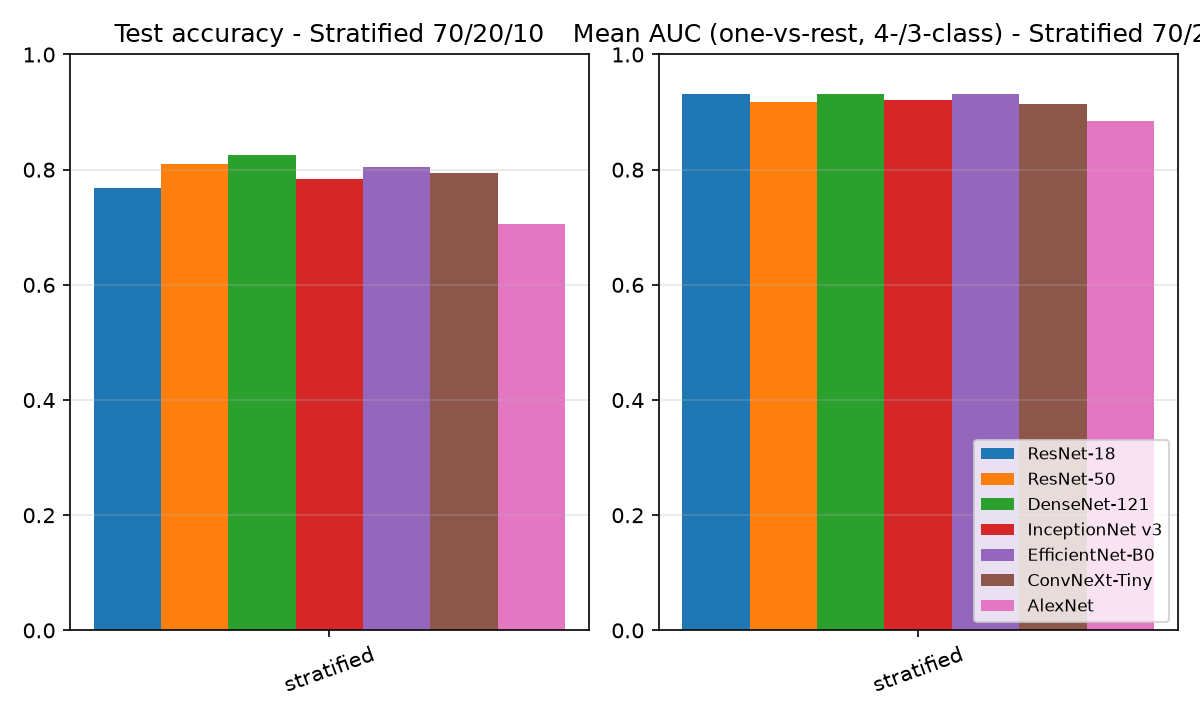
\includegraphics[width=0.75\textwidth]{figures/results/aerobic_zone_stratified_accuracy_auc_bars.png}
    \caption{Test accuracy and mean one-vs-rest AUC of every aerobic zone architecture on the stratified split (Experiment~1).}
    \label{fig:res_mixed_aerobic_bars}
\end{figure}

\subsubsection{Per-Class Precision, Recall and F1}

\begin{table}[htbp]
\centering
\small
\setlength{\tabcolsep}{4pt}
\caption{Per-class precision (P), recall (R) and F1 score of every aerobic zone architecture on the stratified split (Experiment~1).}
\label{tab:res_mixed_aerobic_perclass}
\resizebox{\textwidth}{!}{%
\begin{tabular}{l rrr rrr rrr}
\toprule
& \multicolumn{3}{c}{\textbf{Dysfunctional}} & \multicolumn{3}{c}{\textbf{Functional}} & \multicolumn{3}{c}{\textbf{Suboptimal}} \\
\cmidrule(lr){2-4} \cmidrule(lr){5-7} \cmidrule(lr){8-10}
\textbf{Architecture} & P & R & F1 & P & R & F1 & P & R & F1 \\
\midrule
ResNet-18 & 0.933 & 0.814 & 0.870 & \textbf{0.889} & 0.737 & 0.806 & 0.385 & 0.714 & 0.500 \\
EfficientNet-B0 & 0.973 & 0.849 & \textbf{0.907} & 0.845 & 0.789 & 0.816 & 0.455 & 0.714 & \textbf{0.556} \\
DenseNet-121 & 0.924 & 0.849 & 0.885 & 0.861 & \textbf{0.895} & \textbf{0.877} & \textbf{0.500} & 0.571 & 0.533 \\
ResNet-50 & 0.916 & \textbf{0.884} & 0.899 & 0.863 & 0.829 & 0.846 & 0.441 & 0.536 & 0.484 \\
ConvNeXt-Tiny & \textbf{0.986} & 0.826 & 0.899 & 0.810 & 0.842 & 0.826 & 0.410 & 0.571 & 0.478 \\
Inception-v3 & 0.911 & 0.837 & 0.873 & 0.849 & 0.816 & 0.832 & 0.395 & 0.536 & 0.455 \\
AlexNet & 0.933 & 0.651 & 0.767 & 0.838 & 0.750 & 0.792 & 0.339 & \textbf{0.750} & 0.467 \\
\bottomrule
\end{tabular}}
\end{table}

\subsection{Effect of Augmentation}
\label{sec:results_augmentation}

\begin{table}[htbp]
\centering
\small
\setlength{\tabcolsep}{4pt}
\caption{Test results on the stratified split with (Aug.) and without (None) augmentation during training. $\Delta$ is the difference in percentage points, where a positive value means that augmentation helped.}
\label{tab:res_augmentation}
\begin{tabular}{l rrr rrr rr}
\toprule
& \multicolumn{3}{c}{\textbf{Accuracy}} & \multicolumn{3}{c}{\textbf{Macro F1}} & \multicolumn{2}{c}{\textbf{Mean AUC}} \\
\cmidrule(lr){2-4} \cmidrule(lr){5-7} \cmidrule(lr){8-9}
\textbf{Architecture} & Aug. & None & $\Delta$ & Aug. & None & $\Delta$ & Aug. & None \\
\midrule
\multicolumn{9}{l}{\textit{Clarifiers}} \\
ResNet-18 & 0.854 & 0.850 & +0.4 & 0.864 & 0.875 & -1.1 & 0.961 & 0.955 \\
EfficientNet-B0 & 0.864 & 0.843 & +2.1 & 0.867 & 0.856 & +1.1 & 0.970 & 0.962 \\
DenseNet-121 & 0.882 & 0.843 & +3.9 & 0.880 & 0.818 & +6.2 & 0.975 & 0.958 \\
ResNet-50 & 0.836 & 0.786 & +5.0 & 0.821 & 0.790 & +3.1 & 0.968 & 0.944 \\
ConvNeXt-Tiny & 0.889 & 0.886 & +0.4 & 0.895 & 0.875 & +2.0 & 0.975 & 0.975 \\
Inception-v3 & 0.868 & 0.825 & +4.3 & 0.864 & 0.828 & +3.6 & 0.968 & 0.952 \\
AlexNet & 0.761 & 0.750 & +1.1 & 0.790 & 0.761 & +2.9 & 0.924 & 0.916 \\
\midrule
\multicolumn{9}{l}{\textit{Aerobic zones}} \\
ResNet-18 & 0.768 & 0.795 & -2.6 & 0.725 & 0.736 & -1.0 & 0.931 & 0.929 \\
EfficientNet-B0 & 0.805 & 0.779 & +2.6 & 0.760 & 0.715 & +4.4 & 0.931 & 0.919 \\
DenseNet-121 & 0.826 & 0.795 & +3.2 & 0.765 & 0.750 & +1.5 & 0.932 & 0.909 \\
ResNet-50 & 0.811 & 0.789 & +2.1 & 0.743 & 0.736 & +0.7 & 0.918 & 0.904 \\
ConvNeXt-Tiny & 0.795 & 0.800 & -0.5 & 0.734 & 0.753 & -1.8 & 0.914 & 0.932 \\
Inception-v3 & 0.784 & 0.795 & -1.1 & 0.720 & 0.709 & +1.0 & 0.921 & 0.894 \\
AlexNet & 0.705 & 0.721 & -1.6 & 0.675 & 0.658 & +1.7 & 0.884 & 0.885 \\
\bottomrule
\end{tabular}
\end{table}

\FloatBarrier


\section{Experiment 2: Leave-One-Facility-Out Evaluation}
\label{sec:results_lofo}

\subsection{Clarifiers}
\label{sec:results_lofo_clarifier}

\subsubsection{Comparison Table}

\begin{table}[htbp]
\centering
\small
\setlength{\tabcolsep}{4pt}
\caption{Clarifier test results of every architecture in the leave-one-facility-out experiment (Experiment~2), given as the mean $\pm$ standard deviation across the five held-out facilities.}
\label{tab:res_lofo_clarifier}
\resizebox{\textwidth}{!}{%
\begin{tabular}{lrrrrr}
\toprule
\textbf{Architecture} & \textbf{Accuracy} & \textbf{Mean AUC} & \textbf{\makecell[r]{Macro\\precision}} & \textbf{\makecell[r]{Macro\\recall}} & \textbf{\makecell[r]{Macro\\F1}} \\
\midrule
ResNet-18 & 0.764 $\pm$ 0.097 & 0.914 $\pm$ 0.038 & 0.798 $\pm$ 0.096 & 0.731 $\pm$ 0.092 & 0.739 $\pm$ 0.100 \\
EfficientNet-B0 & 0.804 $\pm$ 0.087 & 0.941 $\pm$ 0.030 & 0.833 $\pm$ 0.105 & 0.747 $\pm$ 0.064 & 0.766 $\pm$ 0.079 \\
DenseNet-121 & 0.802 $\pm$ 0.105 & 0.940 $\pm$ 0.041 & 0.823 $\pm$ 0.100 & 0.742 $\pm$ 0.092 & 0.752 $\pm$ 0.092 \\
ResNet-50 & 0.800 $\pm$ 0.086 & 0.914 $\pm$ 0.039 & 0.815 $\pm$ 0.124 & 0.736 $\pm$ 0.059 & 0.759 $\pm$ 0.088 \\
ConvNeXt-Tiny & \textbf{0.822} $\pm$ 0.080 & \textbf{0.956} $\pm$ 0.018 & \textbf{0.852} $\pm$ 0.088 & \textbf{0.756} $\pm$ 0.079 & \textbf{0.774} $\pm$ 0.077 \\
Inception-v3 & 0.787 $\pm$ 0.106 & 0.920 $\pm$ 0.050 & 0.795 $\pm$ 0.111 & 0.709 $\pm$ 0.073 & 0.719 $\pm$ 0.097 \\
AlexNet & 0.687 $\pm$ 0.104 & 0.863 $\pm$ 0.041 & 0.683 $\pm$ 0.067 & 0.693 $\pm$ 0.060 & 0.665 $\pm$ 0.065 \\
\bottomrule
\end{tabular}}
\end{table}

\subsubsection{Accuracy and AUC Across Facilities}

\begin{figure}[htbp]
    \centering
    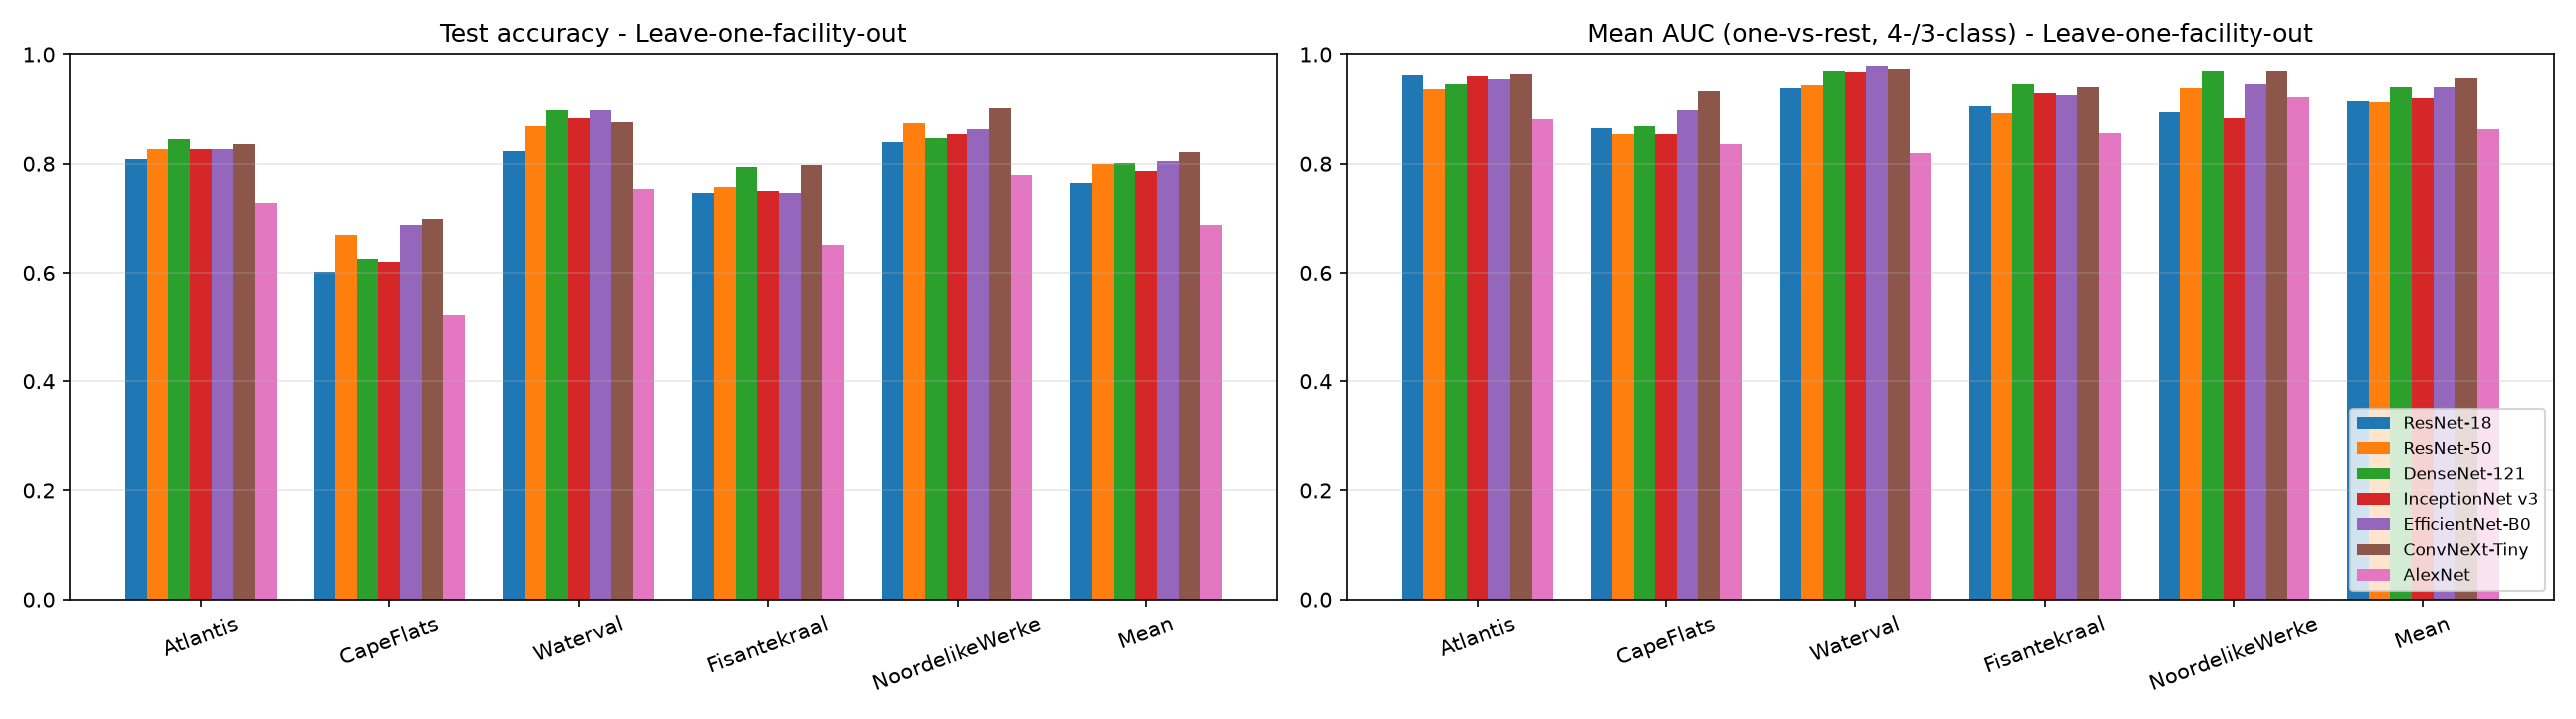
\includegraphics[width=\textwidth]{figures/results/clarifier_lofo_accuracy_auc_bars.png}
    \caption{Test accuracy and mean one-vs-rest AUC of every clarifier architecture for each held-out facility, and the mean across facilities.}
    \label{fig:res_lofo_clarifier_bars}
\end{figure}

\begin{table}[htbp]
\centering
\small
\setlength{\tabcolsep}{4pt}
\caption{Clarifier test accuracy and mean AUC of every architecture for each held-out facility.}
\label{tab:res_lofo_clarifier_facility}
\resizebox{\textwidth}{!}{%
\begin{tabular}{lrrrrrr}
\toprule
\textbf{Architecture} & \textbf{Atlantis} & \textbf{Cape Flats} & \textbf{Fisantekraal} & \textbf{\makecell[r]{Northern\\Works}} & \textbf{Waterval} & \textbf{Mean} \\
\midrule
\multicolumn{7}{l}{\textit{Accuracy}} \\
ResNet-18 & 0.809 & 0.602 & 0.746 & 0.840 & 0.824 & 0.764 \\
EfficientNet-B0 & 0.827 & 0.687 & 0.746 & 0.864 & \textbf{0.898} & 0.804 \\
DenseNet-121 & \textbf{0.845} & 0.626 & 0.794 & 0.847 & \textbf{0.898} & 0.802 \\
ResNet-50 & 0.827 & 0.669 & 0.758 & 0.874 & 0.870 & 0.800 \\
ConvNeXt-Tiny & 0.836 & \textbf{0.699} & \textbf{0.798} & \textbf{0.901} & 0.877 & \textbf{0.822} \\
Inception-v3 & 0.827 & 0.619 & 0.750 & 0.854 & 0.884 & 0.787 \\
AlexNet & 0.727 & 0.523 & 0.651 & 0.780 & 0.754 & 0.687 \\
\midrule
\multicolumn{7}{l}{\textit{Mean AUC}} \\
ResNet-18 & 0.963 & 0.866 & 0.907 & 0.895 & 0.938 & 0.914 \\
EfficientNet-B0 & 0.954 & 0.898 & 0.926 & 0.946 & \textbf{0.978} & 0.941 \\
DenseNet-121 & 0.945 & 0.869 & \textbf{0.946} & 0.970 & 0.970 & 0.940 \\
ResNet-50 & 0.937 & 0.854 & 0.892 & 0.940 & 0.945 & 0.914 \\
ConvNeXt-Tiny & \textbf{0.964} & \textbf{0.932} & 0.941 & \textbf{0.971} & 0.973 & \textbf{0.956} \\
Inception-v3 & 0.961 & 0.854 & 0.930 & 0.884 & 0.969 & 0.920 \\
AlexNet & 0.881 & 0.835 & 0.857 & 0.923 & 0.819 & 0.863 \\
\bottomrule
\end{tabular}}
\end{table}

\subsubsection{Per-Class Precision, Recall and F1}

\begin{table}[htbp]
\centering
\footnotesize
\setlength{\tabcolsep}{3pt}
\caption{Per-class precision (P), recall (R) and F1 score of every clarifier architecture in Experiment~2, averaged over the held-out facilities at which the class occurs.}
\label{tab:res_lofo_clarifier_perclass}
\resizebox{\textwidth}{!}{%
\begin{tabular}{l rrr rrr rrr rrr}
\toprule
& \multicolumn{3}{c}{\textbf{Dysfunctional}} & \multicolumn{3}{c}{\textbf{Empty}} & \multicolumn{3}{c}{\textbf{Functional}} & \multicolumn{3}{c}{\textbf{Scum}} \\
\cmidrule(lr){2-4} \cmidrule(lr){5-7} \cmidrule(lr){8-10} \cmidrule(lr){11-13}
\textbf{Architecture} & P & R & F1 & P & R & F1 & P & R & F1 & P & R & F1 \\
\midrule
ResNet-18 & 0.821 & 0.773 & 0.793 & 0.748 & 0.532 & 0.604 & 0.745 & 0.806 & 0.740 & 0.836 & 0.745 & 0.765 \\
EfficientNet-B0 & 0.839 & 0.767 & 0.796 & 0.837 & 0.586 & 0.652 & 0.802 & 0.790 & 0.778 & 0.827 & 0.812 & 0.809 \\
DenseNet-121 & 0.761 & 0.736 & 0.741 & \textbf{0.863} & 0.564 & 0.630 & 0.816 & 0.791 & 0.774 & 0.835 & 0.808 & 0.806 \\
ResNet-50 & 0.820 & 0.684 & 0.733 & 0.777 & 0.617 & \textbf{0.658} & \textbf{0.820} & 0.781 & 0.791 & 0.805 & 0.808 & 0.803 \\
ConvNeXt-Tiny & \textbf{0.879} & 0.749 & \textbf{0.801} & 0.839 & 0.541 & 0.613 & \textbf{0.820} & \textbf{0.840} & \textbf{0.810} & \textbf{0.853} & \textbf{0.835} & \textbf{0.833} \\
Inception-v3 & 0.866 & 0.685 & 0.754 & 0.626 & 0.495 & 0.482 & 0.791 & 0.812 & 0.779 & 0.832 & 0.779 & 0.789 \\
AlexNet & 0.674 & \textbf{0.814} & 0.732 & 0.628 & \textbf{0.633} & 0.630 & 0.664 & 0.648 & 0.611 & 0.746 & 0.671 & 0.678 \\
\bottomrule
\end{tabular}}
\end{table}

\subsubsection{Training Curves and Confusion Matrices}

\begin{figure}[htbp]
    \centering
    \begin{subfigure}{0.49\textwidth}
        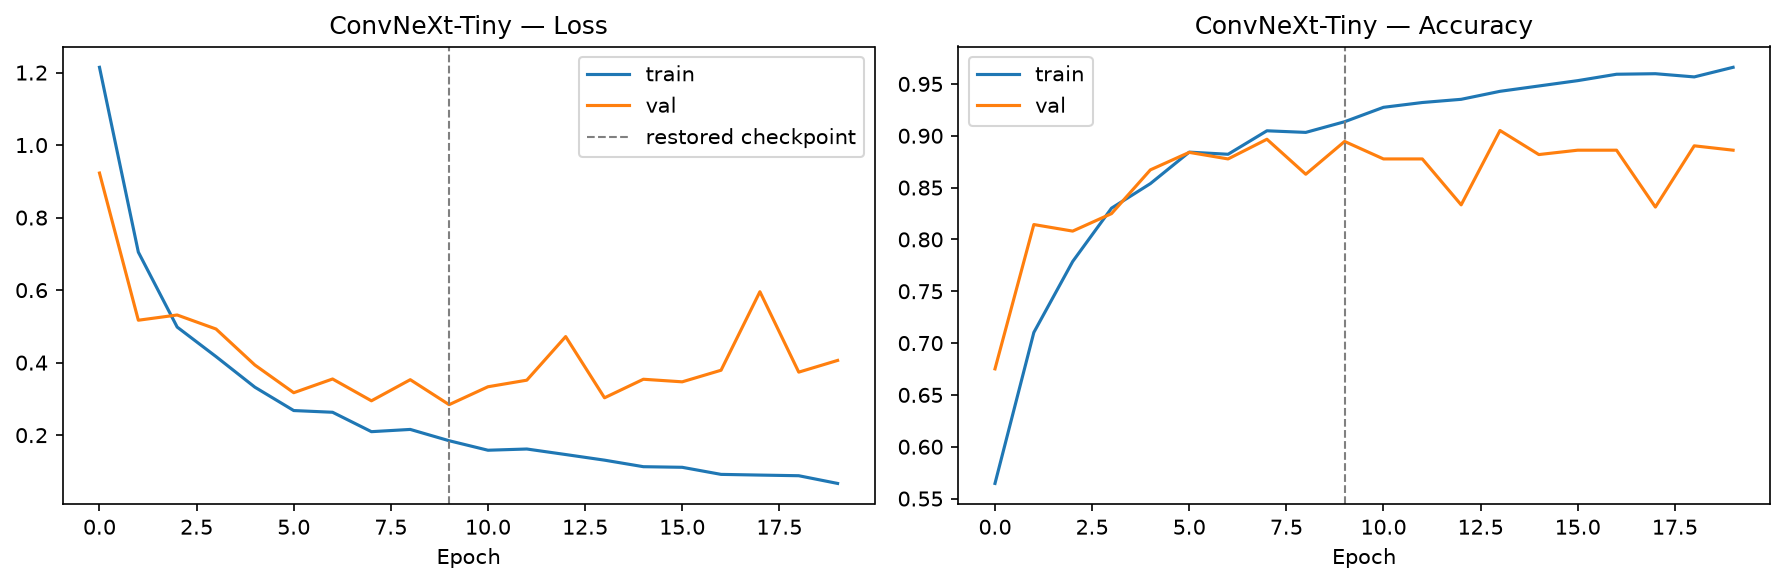
\includegraphics[width=\textwidth]{figures/results/clarifier_convnext_tiny_Atlantis_training_curves.png}
        \caption{Atlantis held out}
    \end{subfigure}
    \hfill
    \begin{subfigure}{0.49\textwidth}
        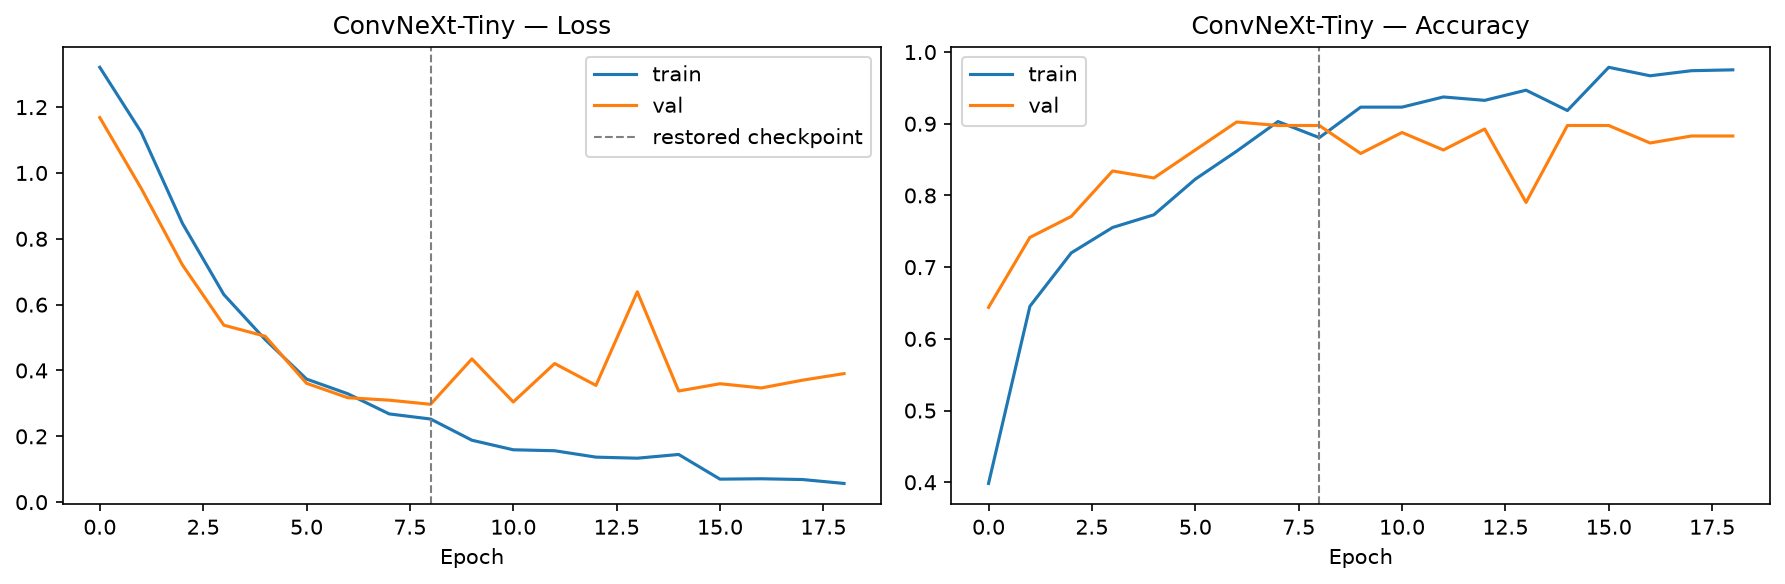
\includegraphics[width=\textwidth]{figures/results/clarifier_convnext_tiny_CapeFlats_training_curves.png}
        \caption{Cape Flats held out}
    \end{subfigure}
    \begin{subfigure}{0.49\textwidth}
        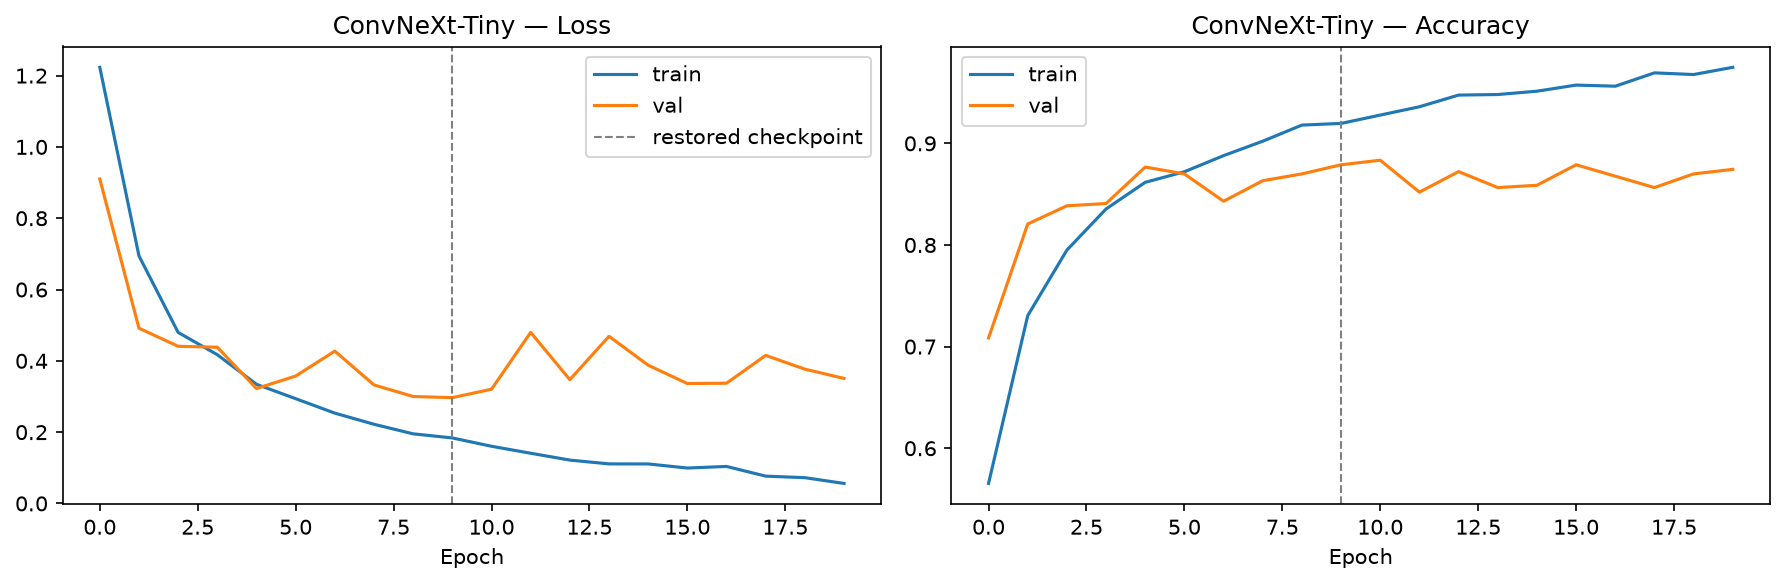
\includegraphics[width=\textwidth]{figures/results/clarifier_convnext_tiny_Fisantekraal_training_curves.png}
        \caption{Fisantekraal held out}
    \end{subfigure}
    \hfill
    \begin{subfigure}{0.49\textwidth}
        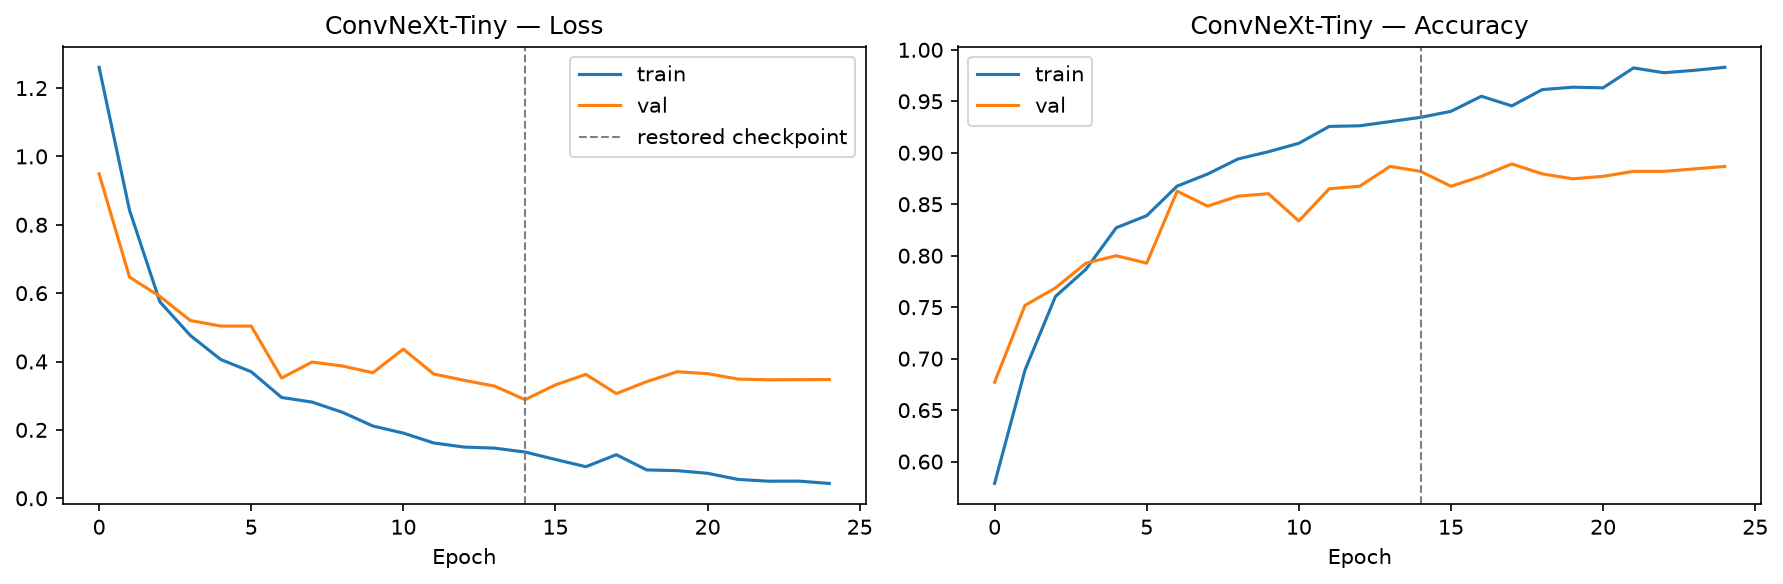
\includegraphics[width=\textwidth]{figures/results/clarifier_convnext_tiny_NoordelikeWerke_training_curves.png}
        \caption{Northern Works held out}
    \end{subfigure}
    \begin{subfigure}{0.49\textwidth}
        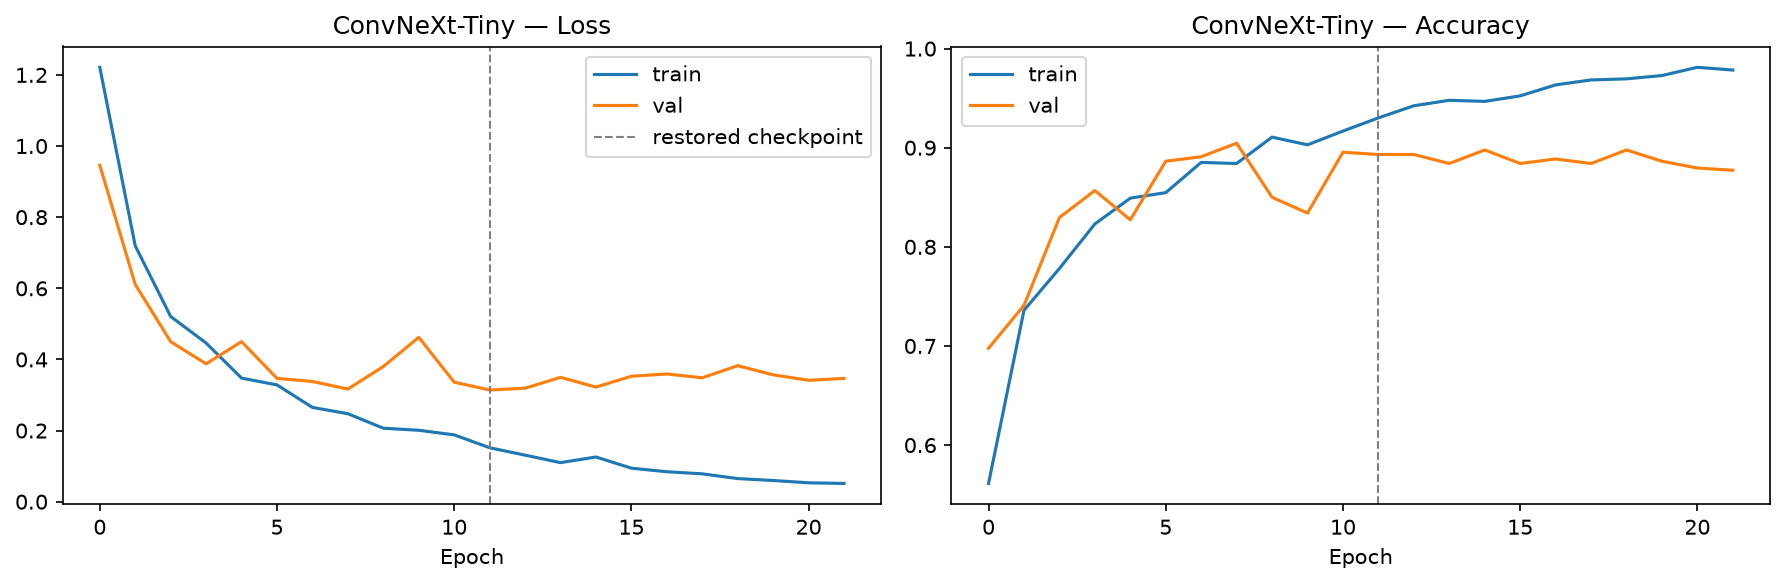
\includegraphics[width=\textwidth]{figures/results/clarifier_convnext_tiny_Waterval_training_curves.png}
        \caption{Waterval held out}
    \end{subfigure}
    \caption{Training and development loss and accuracy of the ConvNeXt-Tiny clarifier model for every leave-one-facility-out fold. The dashed line marks the epoch of the restored checkpoint.}
    \label{fig:res_lofo_clarifier_curves}
\end{figure}

\begin{figure}[htbp]
    \centering
    \begin{subfigure}{0.32\textwidth}
        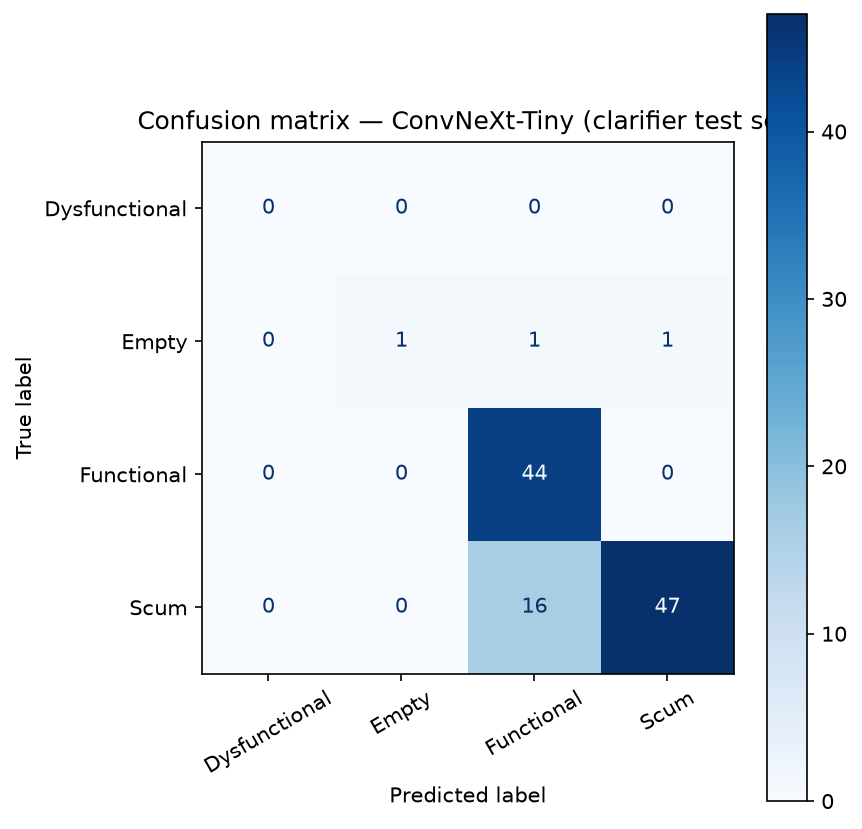
\includegraphics[width=\textwidth]{figures/results/clarifier_convnext_tiny_Atlantis_confusion_matrix.png}
        \caption{Atlantis}
    \end{subfigure}
    \hfill
    \begin{subfigure}{0.32\textwidth}
        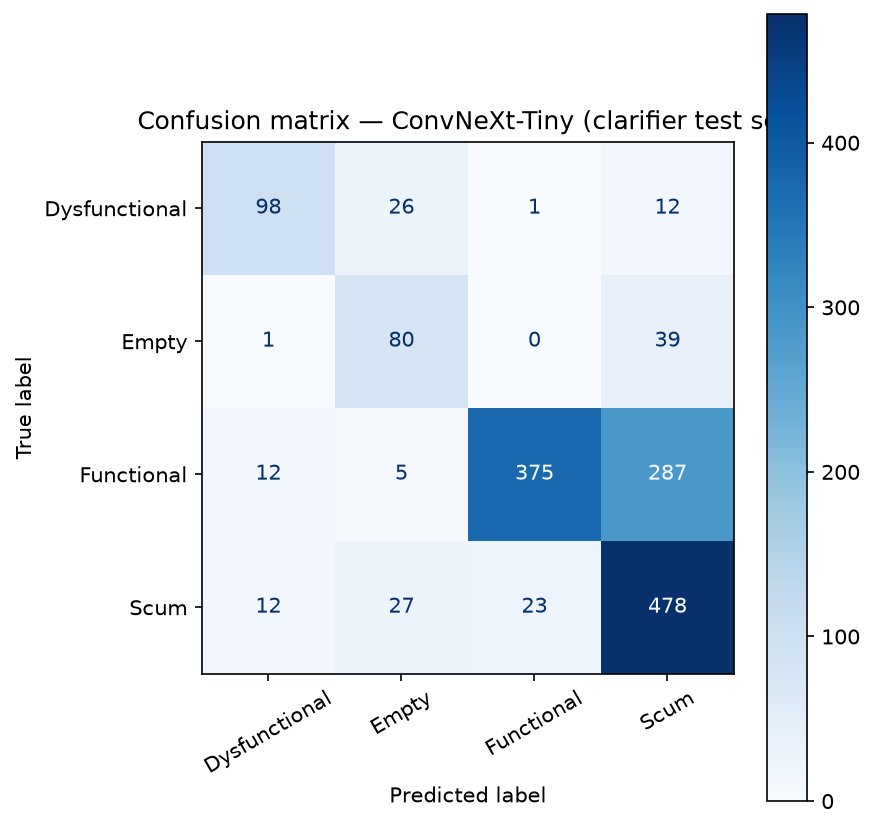
\includegraphics[width=\textwidth]{figures/results/clarifier_convnext_tiny_CapeFlats_confusion_matrix.png}
        \caption{Cape Flats}
    \end{subfigure}
    \hfill
    \begin{subfigure}{0.32\textwidth}
        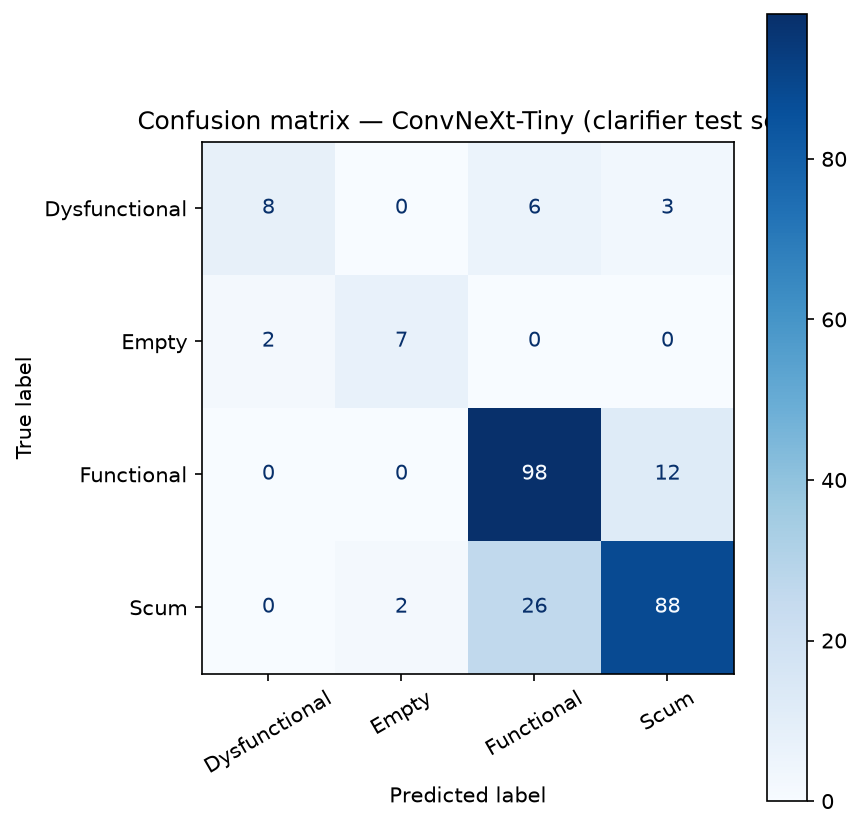
\includegraphics[width=\textwidth]{figures/results/clarifier_convnext_tiny_Fisantekraal_confusion_matrix.png}
        \caption{Fisantekraal}
    \end{subfigure}
    \begin{subfigure}{0.32\textwidth}
        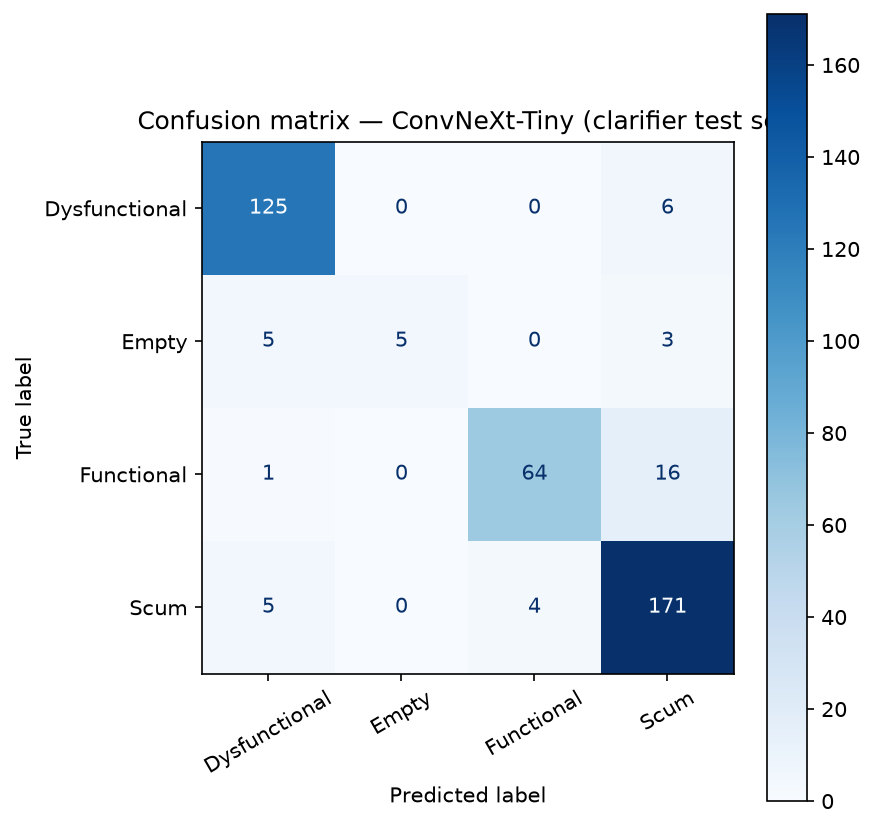
\includegraphics[width=\textwidth]{figures/results/clarifier_convnext_tiny_NoordelikeWerke_confusion_matrix.png}
        \caption{Northern Works}
    \end{subfigure}
    \begin{subfigure}{0.32\textwidth}
        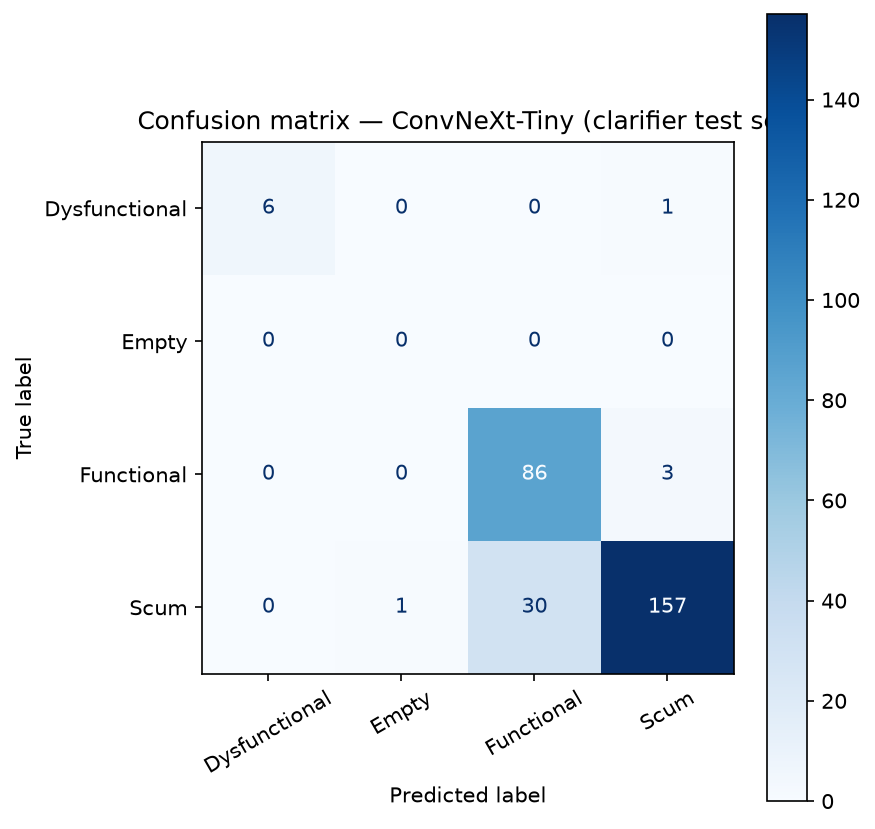
\includegraphics[width=\textwidth]{figures/results/clarifier_convnext_tiny_Waterval_confusion_matrix.png}
        \caption{Waterval}
    \end{subfigure}
    \caption{Confusion matrices of the ConvNeXt-Tiny clarifier model on each held-out facility.}
    \label{fig:res_lofo_clarifier_cm}
\end{figure}

\FloatBarrier

\subsection{Aerobic Zones}
\label{sec:results_lofo_aerobic}

\subsubsection{Comparison Table}

\begin{table}[htbp]
\centering
\small
\setlength{\tabcolsep}{4pt}
\caption{Aerobic zone test results of every architecture in the leave-one-facility-out experiment (Experiment~2), given as the mean $\pm$ standard deviation across the three held-out facilities.}
\label{tab:res_lofo_aerobic}
\resizebox{\textwidth}{!}{%
\begin{tabular}{lrrrrr}
\toprule
\textbf{Architecture} & \textbf{Accuracy} & \textbf{Mean AUC} & \textbf{\makecell[r]{Macro\\precision}} & \textbf{\makecell[r]{Macro\\recall}} & \textbf{\makecell[r]{Macro\\F1}} \\
\midrule
ResNet-18 & 0.611 $\pm$ 0.063 & 0.722 $\pm$ 0.031 & 0.473 $\pm$ 0.033 & 0.498 $\pm$ 0.036 & 0.444 $\pm$ 0.038 \\
EfficientNet-B0 & \textbf{0.629} $\pm$ 0.126 & 0.733 $\pm$ 0.061 & 0.510 $\pm$ 0.043 & 0.505 $\pm$ 0.026 & 0.469 $\pm$ 0.043 \\
DenseNet-121 & 0.592 $\pm$ 0.206 & \textbf{0.775} $\pm$ 0.132 & \textbf{0.554} $\pm$ 0.121 & 0.529 $\pm$ 0.113 & \textbf{0.498} $\pm$ 0.134 \\
ResNet-50 & 0.467 $\pm$ 0.127 & 0.665 $\pm$ 0.050 & 0.444 $\pm$ 0.073 & 0.446 $\pm$ 0.099 & 0.349 $\pm$ 0.102 \\
ConvNeXt-Tiny & 0.558 $\pm$ 0.147 & 0.772 $\pm$ 0.085 & 0.520 $\pm$ 0.077 & \textbf{0.537} $\pm$ 0.057 & 0.474 $\pm$ 0.097 \\
Inception-v3 & 0.567 $\pm$ 0.161 & 0.679 $\pm$ 0.172 & 0.495 $\pm$ 0.135 & 0.492 $\pm$ 0.194 & 0.454 $\pm$ 0.196 \\
AlexNet & 0.370 $\pm$ 0.206 & 0.601 $\pm$ 0.037 & 0.451 $\pm$ 0.078 & 0.389 $\pm$ 0.030 & 0.292 $\pm$ 0.135 \\
\bottomrule
\end{tabular}}
\end{table}

\subsubsection{Accuracy and AUC Across Facilities}

\begin{figure}[htbp]
    \centering
    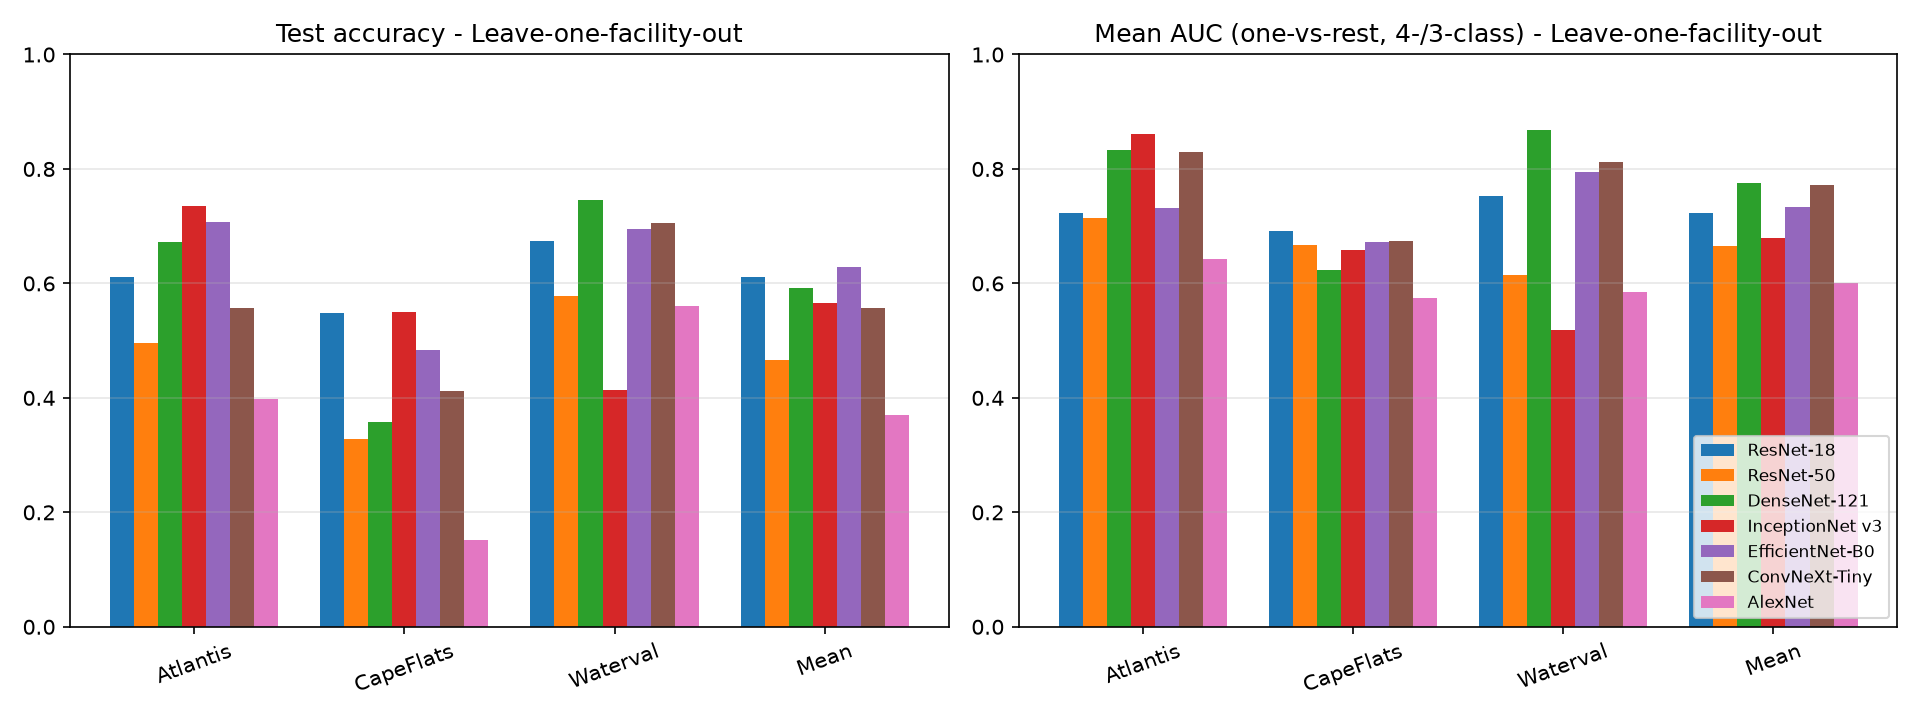
\includegraphics[width=\textwidth]{figures/results/aerobic_zone_lofo_accuracy_auc_bars.png}
    \caption{Test accuracy and mean one-vs-rest AUC of every aerobic zone architecture for each held-out facility, and the mean across facilities.}
    \label{fig:res_lofo_aerobic_bars}
\end{figure}

\begin{table}[htbp]
\centering
\small
\caption{Aerobic zone test accuracy and mean AUC of every architecture for each held-out facility.}
\label{tab:res_lofo_aerobic_facility}
\begin{tabular}{lrrrr}
\toprule
\textbf{Architecture} & \textbf{Atlantis} & \textbf{Cape Flats} & \textbf{Waterval} & \textbf{Mean} \\
\midrule
\multicolumn{5}{l}{\textit{Accuracy}} \\
ResNet-18 & 0.611 & 0.548 & 0.675 & 0.611 \\
EfficientNet-B0 & 0.708 & 0.483 & 0.696 & \textbf{0.629} \\
DenseNet-121 & 0.673 & 0.358 & \textbf{0.747} & 0.592 \\
ResNet-50 & 0.496 & 0.328 & 0.578 & 0.467 \\
ConvNeXt-Tiny & 0.558 & 0.411 & 0.705 & 0.558 \\
Inception-v3 & \textbf{0.735} & \textbf{0.551} & 0.414 & 0.567 \\
AlexNet & 0.398 & 0.151 & 0.561 & 0.370 \\
\midrule
\multicolumn{5}{l}{\textit{Mean AUC}} \\
ResNet-18 & 0.723 & \textbf{0.691} & 0.753 & 0.722 \\
EfficientNet-B0 & 0.731 & 0.673 & 0.795 & 0.733 \\
DenseNet-121 & 0.833 & 0.624 & \textbf{0.869} & \textbf{0.775} \\
ResNet-50 & 0.714 & 0.668 & 0.614 & 0.665 \\
ConvNeXt-Tiny & 0.830 & 0.674 & 0.813 & 0.772 \\
Inception-v3 & \textbf{0.861} & 0.658 & 0.519 & 0.679 \\
AlexNet & 0.643 & 0.575 & 0.585 & 0.601 \\
\bottomrule
\end{tabular}
\end{table}

\subsubsection{Per-Class Precision, Recall and F1}

\begin{table}[htbp]
\centering
\small
\setlength{\tabcolsep}{4pt}
\caption{Per-class precision (P), recall (R) and F1 score of every aerobic zone architecture in Experiment~2, averaged over the three held-out facilities.}
\label{tab:res_lofo_aerobic_perclass}
\resizebox{\textwidth}{!}{%
\begin{tabular}{l rrr rrr rrr}
\toprule
& \multicolumn{3}{c}{\textbf{Dysfunctional}} & \multicolumn{3}{c}{\textbf{Functional}} & \multicolumn{3}{c}{\textbf{Suboptimal}} \\
\cmidrule(lr){2-4} \cmidrule(lr){5-7} \cmidrule(lr){8-10}
\textbf{Architecture} & P & R & F1 & P & R & F1 & P & R & F1 \\
\midrule
ResNet-18 & 0.599 & 0.578 & 0.558 & 0.616 & \textbf{0.820} & 0.654 & 0.204 & 0.096 & 0.121 \\
EfficientNet-B0 & 0.624 & \textbf{0.582} & \textbf{0.575} & 0.655 & 0.747 & \textbf{0.691} & 0.250 & 0.185 & 0.141 \\
DenseNet-121 & \textbf{0.719} & 0.557 & 0.569 & 0.648 & 0.762 & 0.682 & \textbf{0.294} & 0.268 & 0.244 \\
ResNet-50 & 0.591 & 0.477 & 0.395 & 0.602 & 0.729 & 0.524 & 0.140 & 0.130 & 0.126 \\
ConvNeXt-Tiny & 0.690 & 0.573 & 0.551 & \textbf{0.669} & 0.739 & 0.635 & 0.201 & 0.298 & 0.237 \\
Inception-v3 & 0.662 & 0.502 & 0.497 & 0.595 & 0.632 & 0.600 & 0.227 & \textbf{0.341} & \textbf{0.263} \\
AlexNet & 0.693 & 0.163 & 0.204 & 0.547 & 0.715 & 0.512 & 0.113 & 0.288 & 0.160 \\
\bottomrule
\end{tabular}}
\end{table}

\subsubsection{Training Curves and Confusion Matrices}

\begin{figure}[htbp]
    \centering
    \begin{subfigure}{0.49\textwidth}
        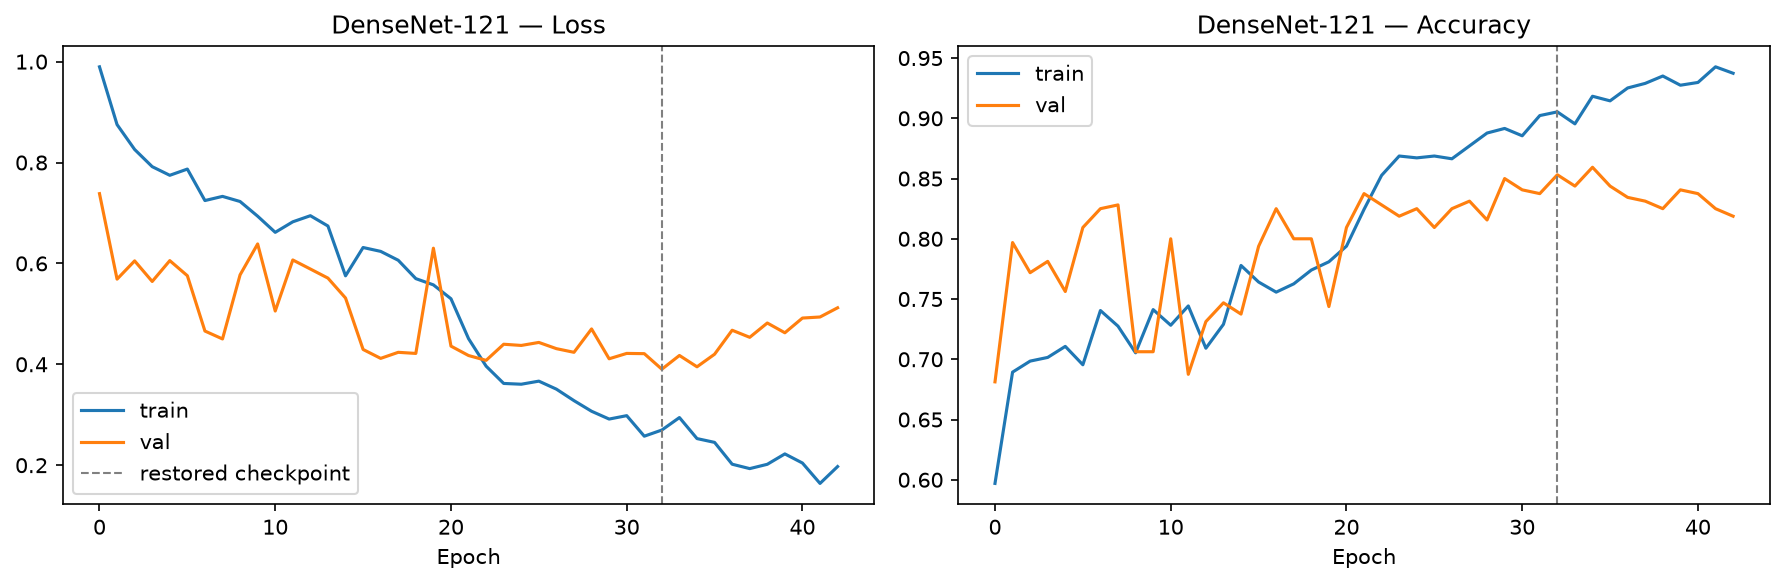
\includegraphics[width=\textwidth]{figures/results/aerobic_zone_densenet_121_Atlantis_training_curves.png}
        \caption{Atlantis held out}
    \end{subfigure}
    \hfill
    \begin{subfigure}{0.49\textwidth}
        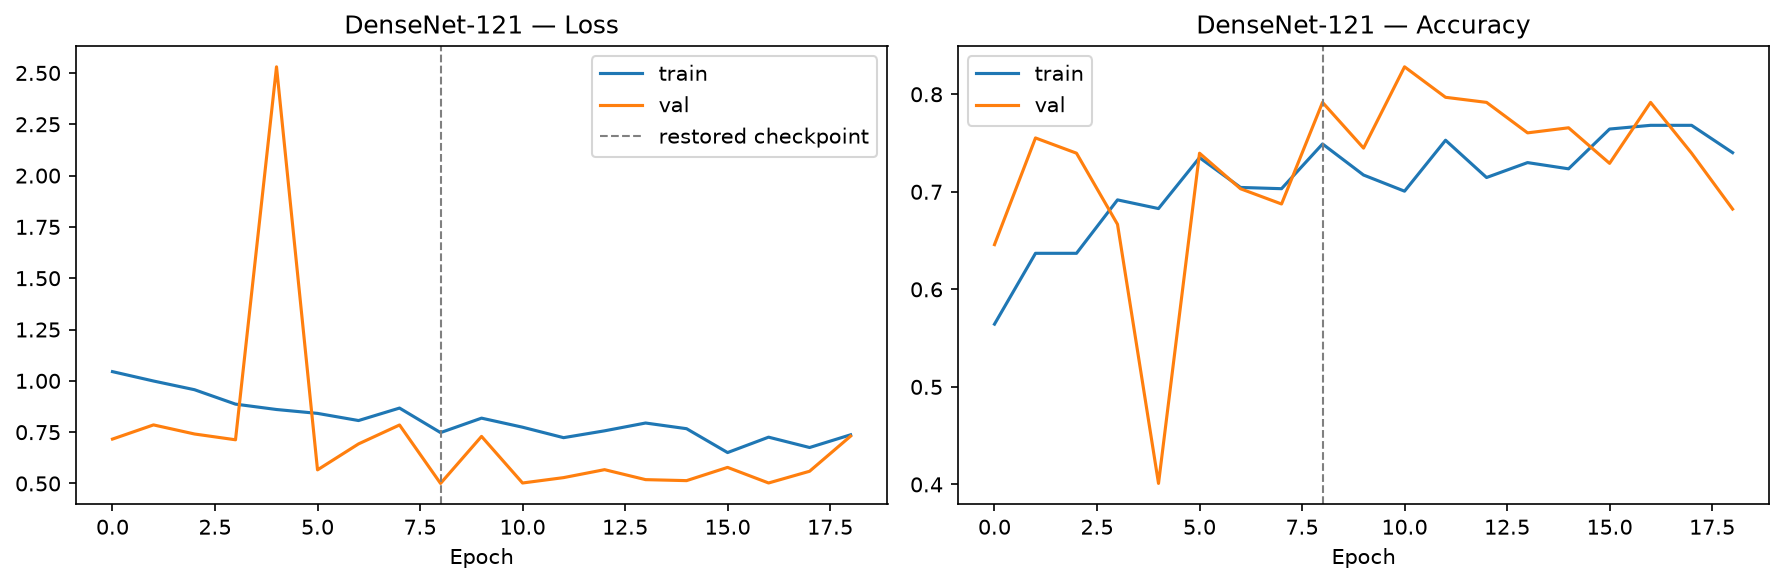
\includegraphics[width=\textwidth]{figures/results/aerobic_zone_densenet_121_CapeFlats_training_curves.png}
        \caption{Cape Flats held out}
    \end{subfigure}
    \begin{subfigure}{0.49\textwidth}
        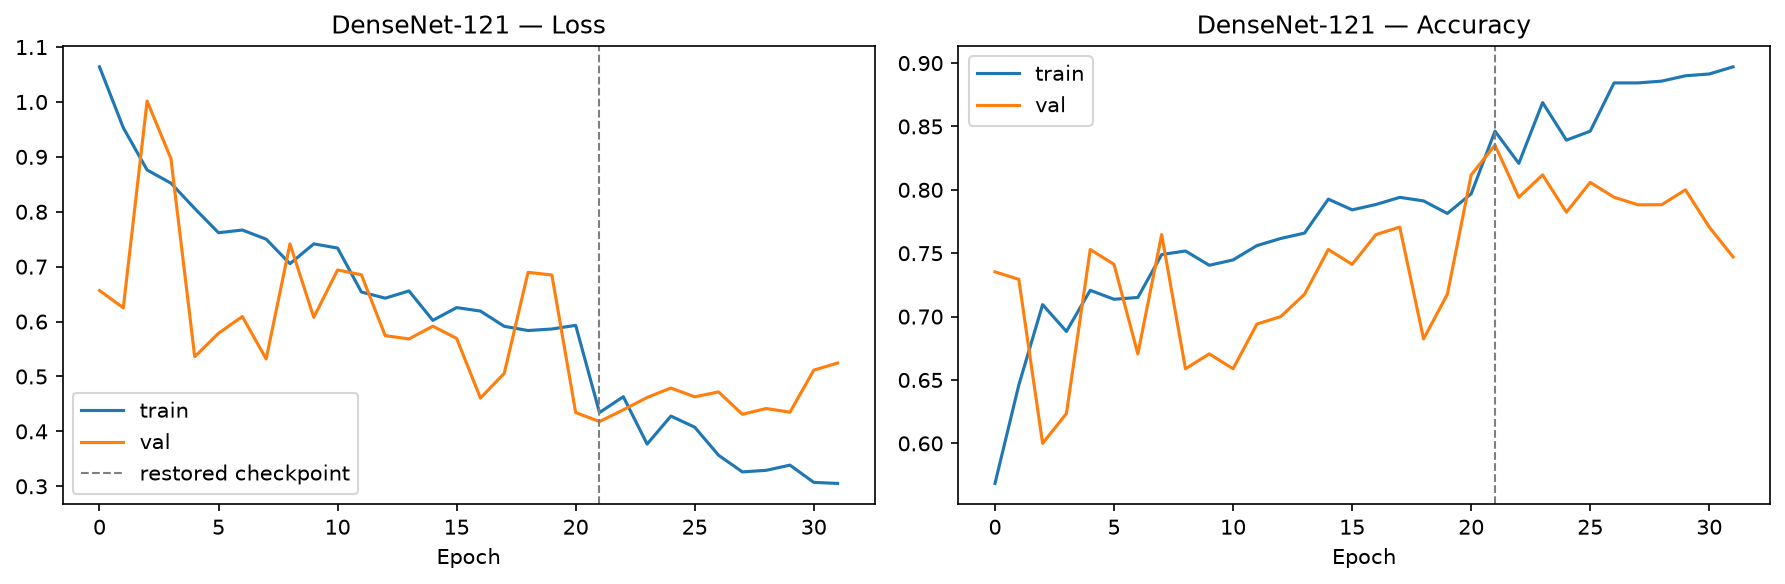
\includegraphics[width=\textwidth]{figures/results/aerobic_zone_densenet_121_Waterval_training_curves.png}
        \caption{Waterval held out}
    \end{subfigure}
    \caption{Training and development loss and accuracy of the DenseNet-121 aerobic zone model for every leave-one-facility-out fold. The dashed line marks the epoch of the restored checkpoint.}
    \label{fig:res_lofo_aerobic_curves}
\end{figure}

\begin{figure}[htbp]
    \centering
    \begin{subfigure}{0.32\textwidth}
        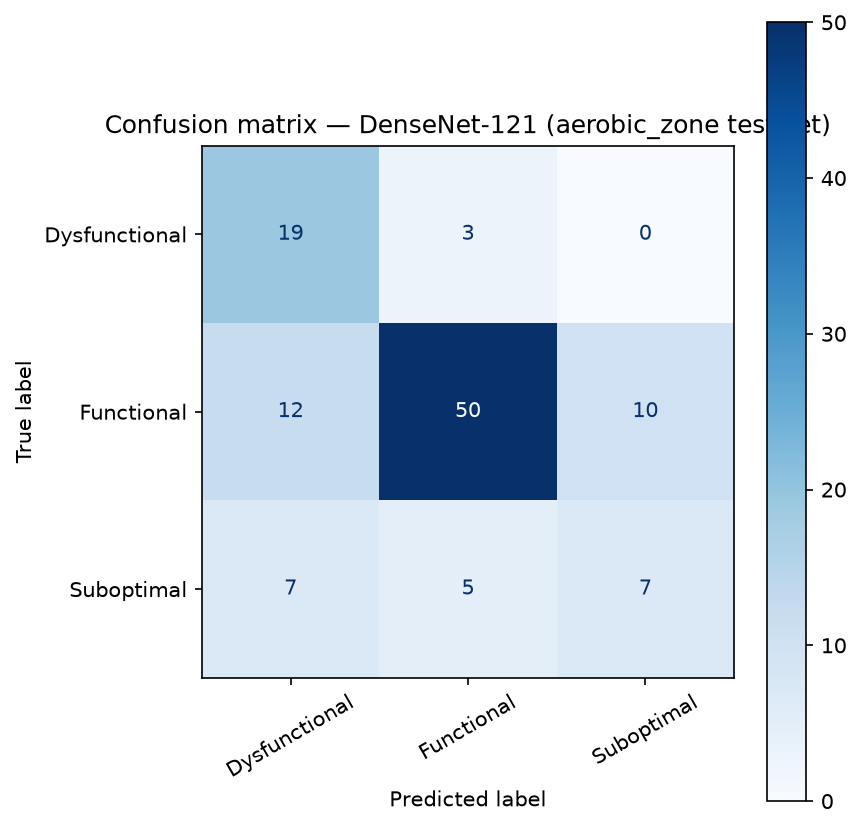
\includegraphics[width=\textwidth]{figures/results/aerobic_zone_densenet_121_Atlantis_confusion_matrix.png}
        \caption{Atlantis}
    \end{subfigure}
    \hfill
    \begin{subfigure}{0.32\textwidth}
        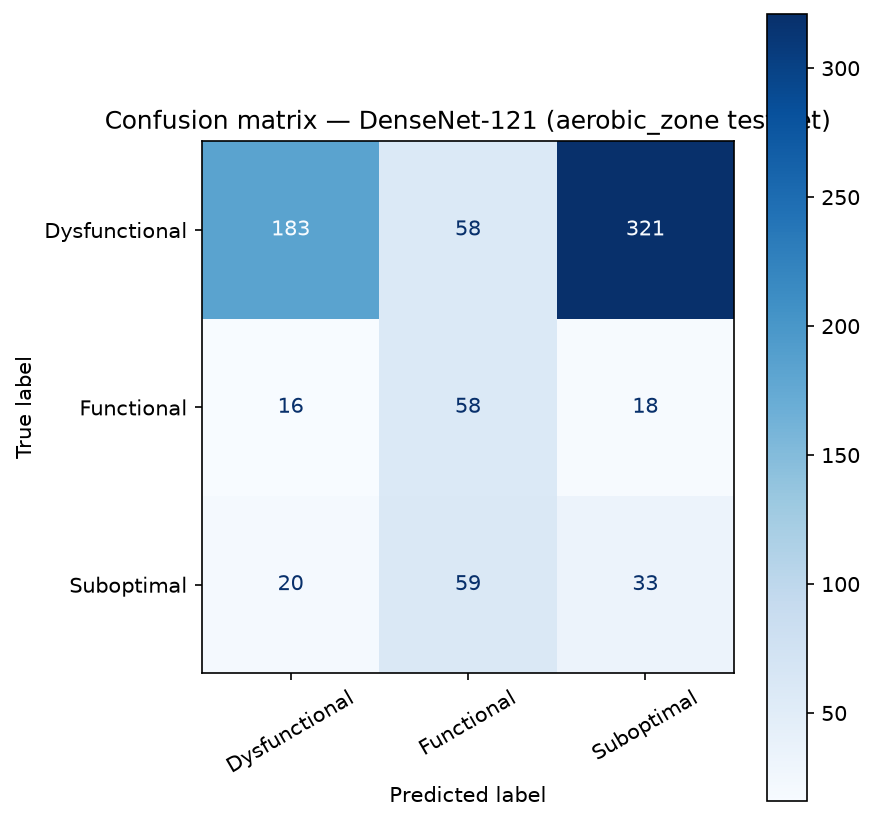
\includegraphics[width=\textwidth]{figures/results/aerobic_zone_densenet_121_CapeFlats_confusion_matrix.png}
        \caption{Cape Flats}
    \end{subfigure}
    \hfill
    \begin{subfigure}{0.32\textwidth}
        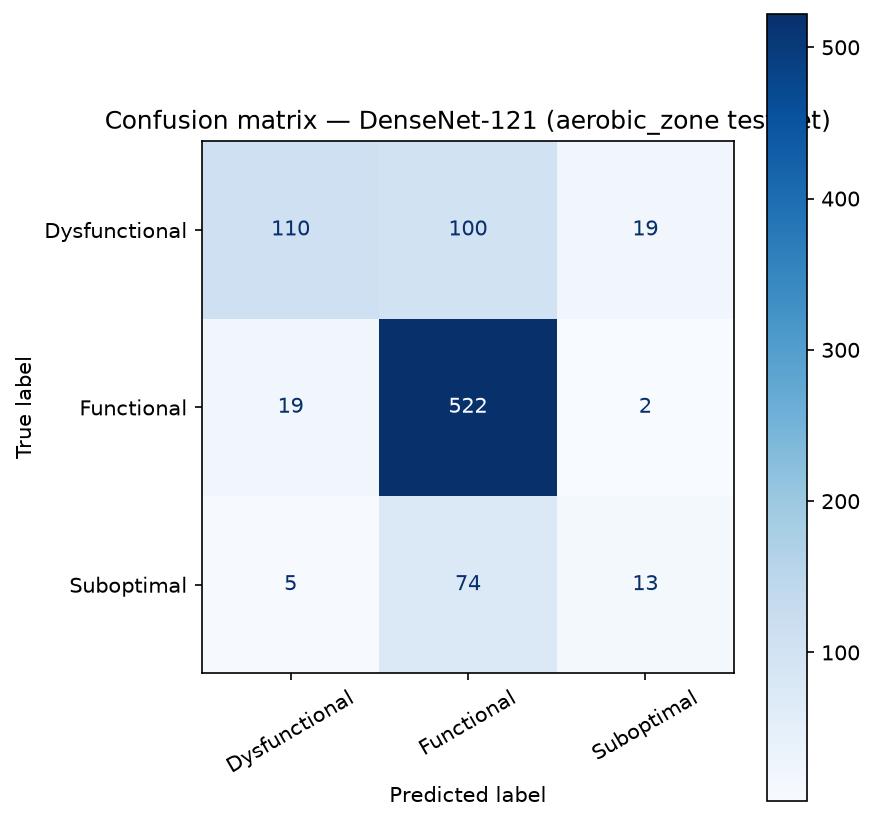
\includegraphics[width=\textwidth]{figures/results/aerobic_zone_densenet_121_Waterval_confusion_matrix.png}
        \caption{Waterval}
    \end{subfigure}
    \caption{Confusion matrices of the DenseNet-121 aerobic zone model on each held-out facility.}
    \label{fig:res_lofo_aerobic_cm}
\end{figure}

\FloatBarrier

\subsection{Generalisation: Mixed-Facility Baseline vs Leave-One-Facility-Out}
\label{sec:results_generalisation}

\begin{table}[htbp]
\centering
\small
\caption{Test accuracy and macro F1 score on the stratified split (Experiment~1) and the mean across held-out facilities (Experiment~2). $\Delta$ is the change in percentage points from Experiment~1 to Experiment~2.}
\label{tab:res_generalisation}
\begin{tabular}{l rrr rrr}
\toprule
& \multicolumn{3}{c}{\textbf{Accuracy}} & \multicolumn{3}{c}{\textbf{Macro F1}} \\
\cmidrule(lr){2-4} \cmidrule(lr){5-7}
\textbf{Architecture} & Exp.~1 & Exp.~2 & $\Delta$ & Exp.~1 & Exp.~2 & $\Delta$ \\
\midrule
\multicolumn{7}{l}{\textit{Clarifiers}} \\
ResNet-18 & 0.854 & 0.764 & -8.9 & 0.864 & 0.739 & -12.5 \\
EfficientNet-B0 & 0.864 & 0.804 & -6.0 & 0.867 & 0.766 & -10.1 \\
DenseNet-121 & 0.882 & 0.802 & -8.0 & 0.880 & 0.752 & -12.8 \\
ResNet-50 & 0.836 & 0.800 & -3.6 & 0.821 & 0.759 & -6.2 \\
ConvNeXt-Tiny & 0.889 & 0.822 & -6.7 & 0.895 & 0.774 & -12.1 \\
Inception-v3 & 0.868 & 0.787 & -8.1 & 0.864 & 0.719 & -14.6 \\
AlexNet & 0.761 & 0.687 & -7.4 & 0.790 & 0.665 & -12.5 \\
\midrule
\multicolumn{7}{l}{\textit{Aerobic zones}} \\
ResNet-18 & 0.768 & 0.611 & -15.7 & 0.725 & 0.444 & -28.1 \\
EfficientNet-B0 & 0.805 & 0.629 & -17.6 & 0.760 & 0.469 & -29.0 \\
DenseNet-121 & 0.826 & 0.592 & -23.4 & 0.765 & 0.498 & -26.7 \\
ResNet-50 & 0.811 & 0.467 & -34.4 & 0.743 & 0.349 & -39.4 \\
ConvNeXt-Tiny & 0.795 & 0.558 & -23.7 & 0.734 & 0.474 & -26.0 \\
Inception-v3 & 0.784 & 0.567 & -21.8 & 0.720 & 0.454 & -26.6 \\
AlexNet & 0.705 & 0.370 & -33.5 & 0.675 & 0.292 & -38.3 \\
\bottomrule
\end{tabular}
\end{table}

\subsection{Hue Shift}
\label{sec:results_hue_ablation}

To check whether the hue shift in the colour jitter augmentation (Section~\ref{sec:exp_augmentation}) was washing out the green surface that identifies a \textbf{Dysfunctional} clarifier, all seven clarifier architectures were retrained on all five leave-one-facility-out splits with the hue shift disabled, keeping every other augmentation and hyperparameter the same. This did not improve performance: the mean test accuracy decreased for every architecture, by between 0.1 and 3.1 percentage points for the six pretrained architectures, and the number of correctly identified \textbf{Dysfunctional} clarifiers did not improve consistently. The hue shift was therefore kept for both components (Section~\ref{sec:exp_augmentation}).

% NOTE: these runs come from an earlier training round (results/archive/phase3_tuned_aug_hue0.1 and
% phase4_tuned_aug_hue0), made before the supervisor's relabelling review, which is why the number of
% Dysfunctional test clarifiers (273) differs from Table~\ref{tab:lofo_folds} (292).
\begin{table}[htbp]
\centering
\small
\caption{Mean clarifier test accuracy across the five held-out facilities, and the total number of correctly classified \textbf{Dysfunctional} clarifiers (out of 273), with and without the hue shift. $\Delta$ is the change in percentage points when the hue shift is removed. These runs were made before the clarifier labels were reviewed.}
\label{tab:res_hue}
\begin{tabular}{l rrr rr}
\toprule
& \multicolumn{3}{c}{\textbf{Mean accuracy}} & \multicolumn{2}{c}{\textbf{Correct Dysfunctional}} \\
\cmidrule(lr){2-4} \cmidrule(lr){5-6}
\textbf{Architecture} & With & Without & $\Delta$ & With & Without \\
\midrule
ResNet-18 & 0.782 & 0.754 & -2.8 & 216 & 215 \\
EfficientNet-B0 & 0.806 & 0.791 & -1.5 & 212 & 213 \\
DenseNet-121 & 0.814 & 0.783 & -3.1 & 216 & 204 \\
ResNet-50 & 0.801 & 0.777 & -2.5 & 214 & 187 \\
ConvNeXt-Tiny & 0.842 & 0.829 & -1.3 & 226 & 230 \\
Inception-v3 & 0.777 & 0.777 & -0.1 & 200 & 212 \\
AlexNet & 0.496 & 0.355 & -14.0 & 7 & 31 \\
\bottomrule
\end{tabular}
\end{table}

\FloatBarrier


\section{Experiment 3: Binary (OK / Not-OK) Reformulation}
\label{sec:results_binary}

\subsection{Clarifiers}
\label{sec:results_binary_clarifier}

\begin{table}[htbp]
\centering
\caption{Binary OK / Not-OK AUC of every clarifier architecture on the stratified split, and the mean $\pm$ standard deviation across held-out facilities.}
\label{tab:res_binary_clarifier}
\begin{tabular}{lrr}
\toprule
\textbf{Architecture} & \textbf{Stratified} & \textbf{Leave-one-facility-out} \\
\midrule
ResNet-18 & 0.960 & 0.921 $\pm$ 0.045 \\
EfficientNet-B0 & 0.961 & 0.935 $\pm$ 0.038 \\
DenseNet-121 & \textbf{0.977} & 0.941 $\pm$ 0.035 \\
ResNet-50 & 0.962 & 0.927 $\pm$ 0.036 \\
ConvNeXt-Tiny & 0.975 & \textbf{0.953} $\pm$ 0.031 \\
Inception-v3 & 0.968 & 0.934 $\pm$ 0.034 \\
AlexNet & 0.910 & 0.844 $\pm$ 0.059 \\
\bottomrule
\end{tabular}
\end{table}

\begin{figure}[htbp]
    \centering
    \begin{subfigure}{0.49\textwidth}
        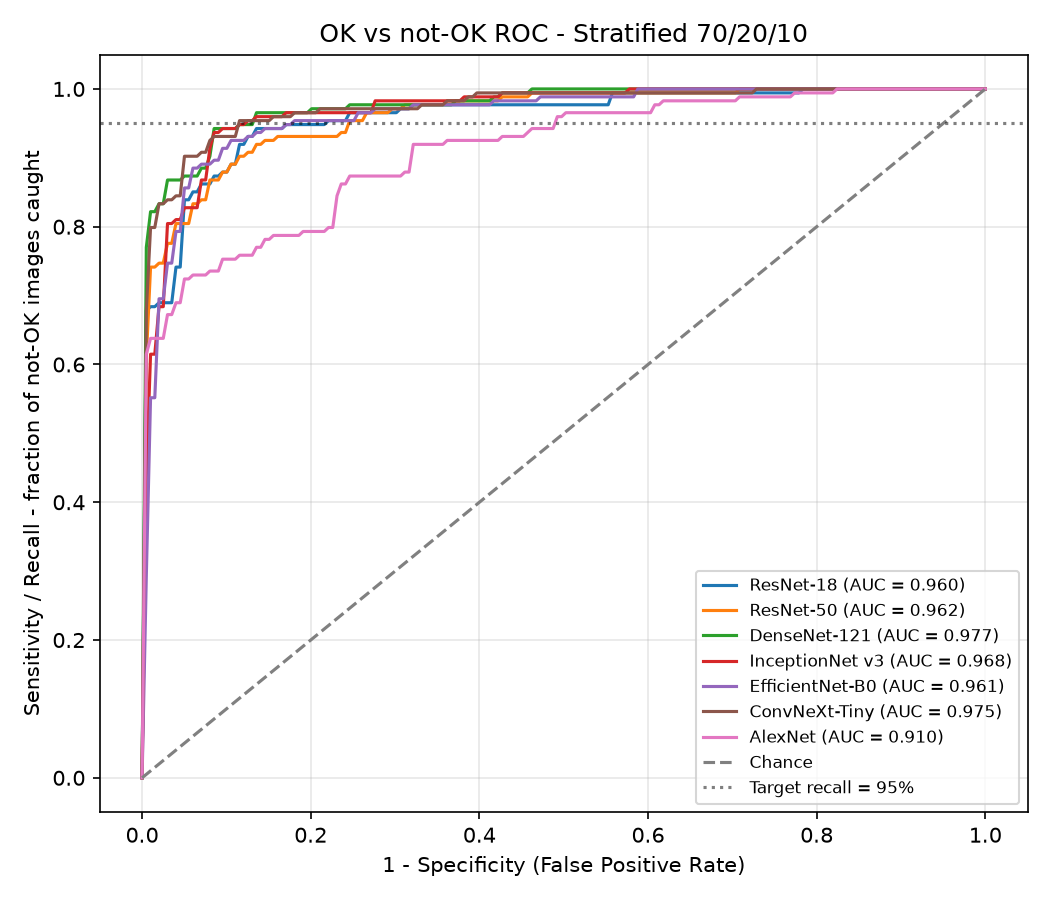
\includegraphics[width=\textwidth]{figures/results/clarifier_stratified_ok_vs_notok_roc.png}
        \caption{Stratified split}
    \end{subfigure}
    \hfill
    \begin{subfigure}{0.49\textwidth}
        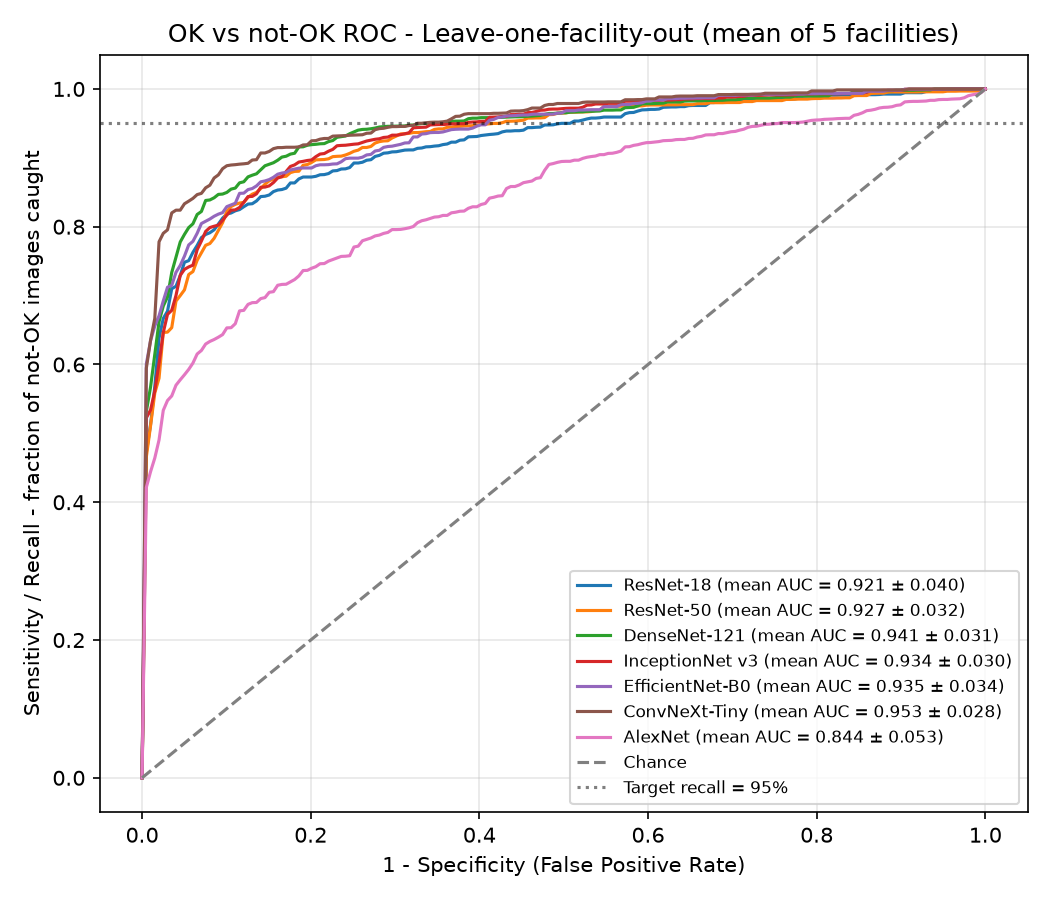
\includegraphics[width=\textwidth]{figures/results/clarifier_lofo_ok_vs_notok_roc.png}
        \caption{Leave-one-facility-out (mean)}
    \end{subfigure}
    \caption{Binary OK / Not-OK ROC curves of the clarifier models. The dotted line marks the 95\% target recall. The legend in (b) gives the population standard deviation, so it differs slightly from Table~\ref{tab:res_binary_clarifier}.}
    \label{fig:res_binary_clarifier_roc}
\end{figure}

\subsection{Aerobic Zones}
\label{sec:results_binary_aerobic}

\begin{table}[htbp]
\centering
\caption{Binary OK / Not-OK AUC of every aerobic zone architecture on the stratified split, and the mean $\pm$ standard deviation across held-out facilities.}
\label{tab:res_binary_aerobic}
\begin{tabular}{lrr}
\toprule
\textbf{Architecture} & \textbf{Stratified} & \textbf{Leave-one-facility-out} \\
\midrule
ResNet-18 & 0.954 & 0.846 $\pm$ 0.036 \\
EfficientNet-B0 & 0.947 & 0.829 $\pm$ 0.029 \\
DenseNet-121 & \textbf{0.959} & 0.865 $\pm$ 0.030 \\
ResNet-50 & 0.956 & 0.759 $\pm$ 0.123 \\
ConvNeXt-Tiny & 0.947 & \textbf{0.866} $\pm$ 0.038 \\
Inception-v3 & 0.950 & 0.705 $\pm$ 0.221 \\
AlexNet & 0.917 & 0.688 $\pm$ 0.071 \\
\bottomrule
\end{tabular}
\end{table}

\begin{figure}[htbp]
    \centering
    \begin{subfigure}{0.49\textwidth}
        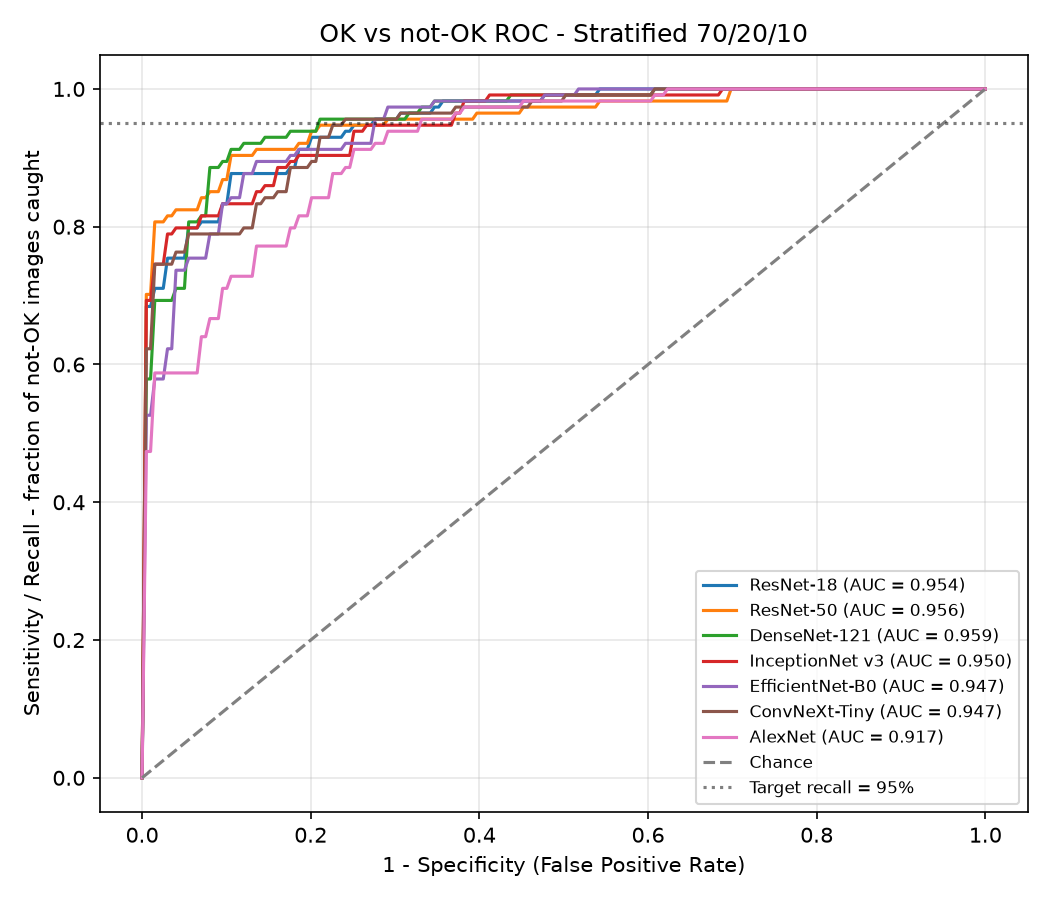
\includegraphics[width=\textwidth]{figures/results/aerobic_zone_stratified_ok_vs_notok_roc.png}
        \caption{Stratified split}
    \end{subfigure}
    \hfill
    \begin{subfigure}{0.49\textwidth}
        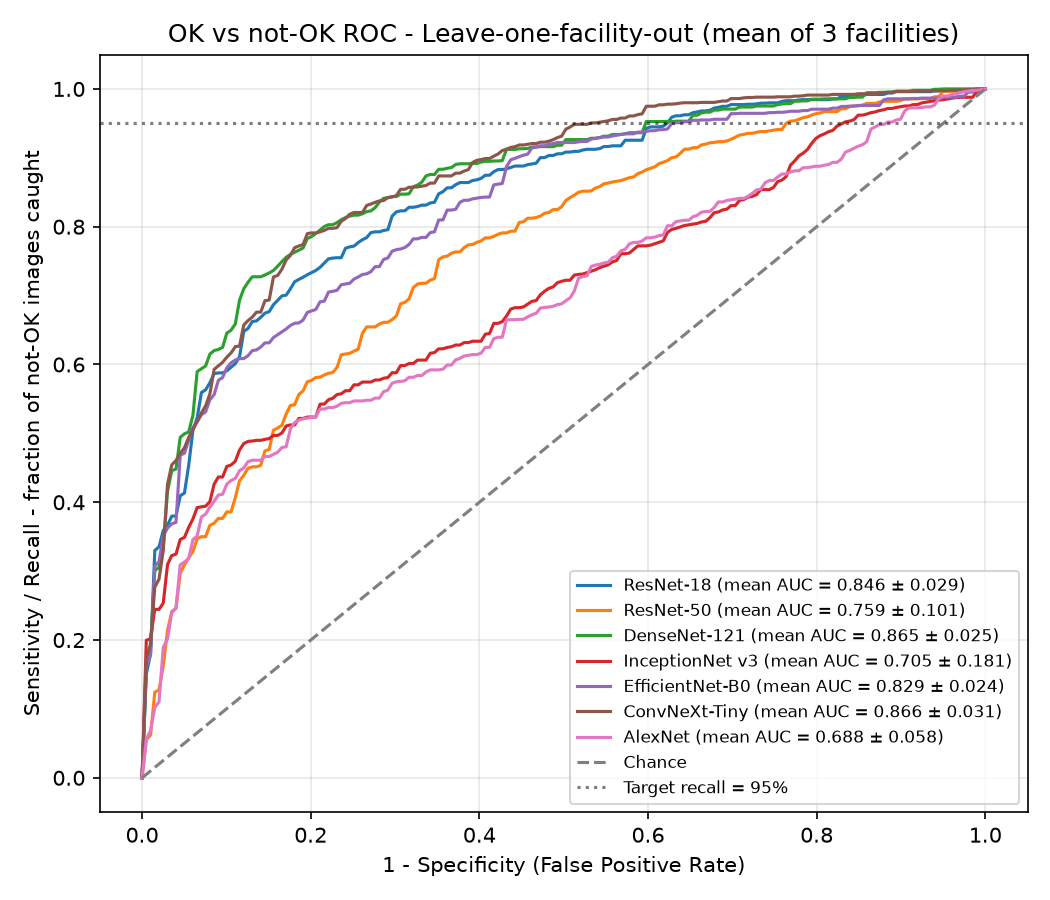
\includegraphics[width=\textwidth]{figures/results/aerobic_zone_lofo_ok_vs_notok_roc.png}
        \caption{Leave-one-facility-out (mean)}
    \end{subfigure}
    \caption{Binary OK / Not-OK ROC curves of the aerobic zone models. The dotted line marks the 95\% target recall.}
    \label{fig:res_binary_aerobic_roc}
\end{figure}

\FloatBarrier

\subsection{Choosing an Operating Threshold}
\label{sec:results_threshold}

\begin{table}[htbp]
\centering
\small
\setlength{\tabcolsep}{4pt}
\caption{Threshold $t$ on the Not-OK score chosen for a 95\% recall, with the recall, specificity and precision of the Not-OK class at that threshold. For the leave-one-facility-out split, one threshold is shared by all folds and the metrics are averaged across held-out facilities.}
\label{tab:res_threshold}
\begin{tabular}{l rrrr rrrr}
\toprule
& \multicolumn{4}{c}{\textbf{Stratified}} & \multicolumn{4}{c}{\textbf{Leave-one-facility-out}} \\
\cmidrule(lr){2-5} \cmidrule(lr){6-9}
\textbf{Architecture} & $t$ & Recall & Spec. & Prec. & $t$ & Recall & Spec. & Prec. \\
\midrule
\multicolumn{9}{l}{\textit{Clarifiers}} \\
ResNet-18 & 0.261 & 0.954 & 0.783 & 0.878 & 0.084 & 0.951 & 0.441 & 0.768 \\
EfficientNet-B0 & 0.289 & 0.954 & 0.821 & 0.897 & 0.154 & 0.951 & 0.480 & 0.784 \\
DenseNet-121 & 0.329 & 0.954 & 0.868 & 0.922 & 0.062 & 0.950 & 0.432 & 0.780 \\
ResNet-50 & 0.072 & 0.954 & 0.755 & 0.865 & 0.168 & 0.953 & 0.524 & 0.788 \\
ConvNeXt-Tiny & 0.240 & 0.954 & 0.877 & 0.927 & 0.110 & 0.950 & 0.528 & 0.797 \\
Inception-v3 & 0.325 & 0.954 & 0.877 & 0.927 & 0.102 & 0.952 & 0.511 & 0.794 \\
AlexNet & 0.257 & 0.954 & 0.509 & 0.761 & 0.144 & 0.953 & 0.190 & 0.685 \\
\midrule
\multicolumn{9}{l}{\textit{Aerobic zones}} \\
ResNet-18 & 0.571 & 0.956 & 0.724 & 0.838 & 0.100 & 0.950 & 0.269 & 0.574 \\
EfficientNet-B0 & 0.343 & 0.956 & 0.724 & 0.838 & 0.236 & 0.957 & 0.325 & 0.614 \\
DenseNet-121 & 0.387 & 0.956 & 0.776 & 0.865 & 0.158 & 0.952 & 0.408 & 0.665 \\
ResNet-50 & 0.222 & 0.956 & 0.711 & 0.832 & 0.134 & 0.952 & 0.168 & 0.557 \\
ConvNeXt-Tiny & 0.144 & 0.956 & 0.763 & 0.858 & 0.074 & 0.951 & 0.409 & 0.634 \\
Inception-v3 & 0.086 & 0.956 & 0.632 & 0.796 & 0.146 & 0.950 & 0.259 & 0.602 \\
AlexNet & 0.385 & 0.956 & 0.671 & 0.813 & 0.150 & 0.953 & 0.137 & 0.551 \\
\bottomrule
\end{tabular}
\end{table}

\begin{figure}[htbp]
    \centering
    \begin{subfigure}{\textwidth}
        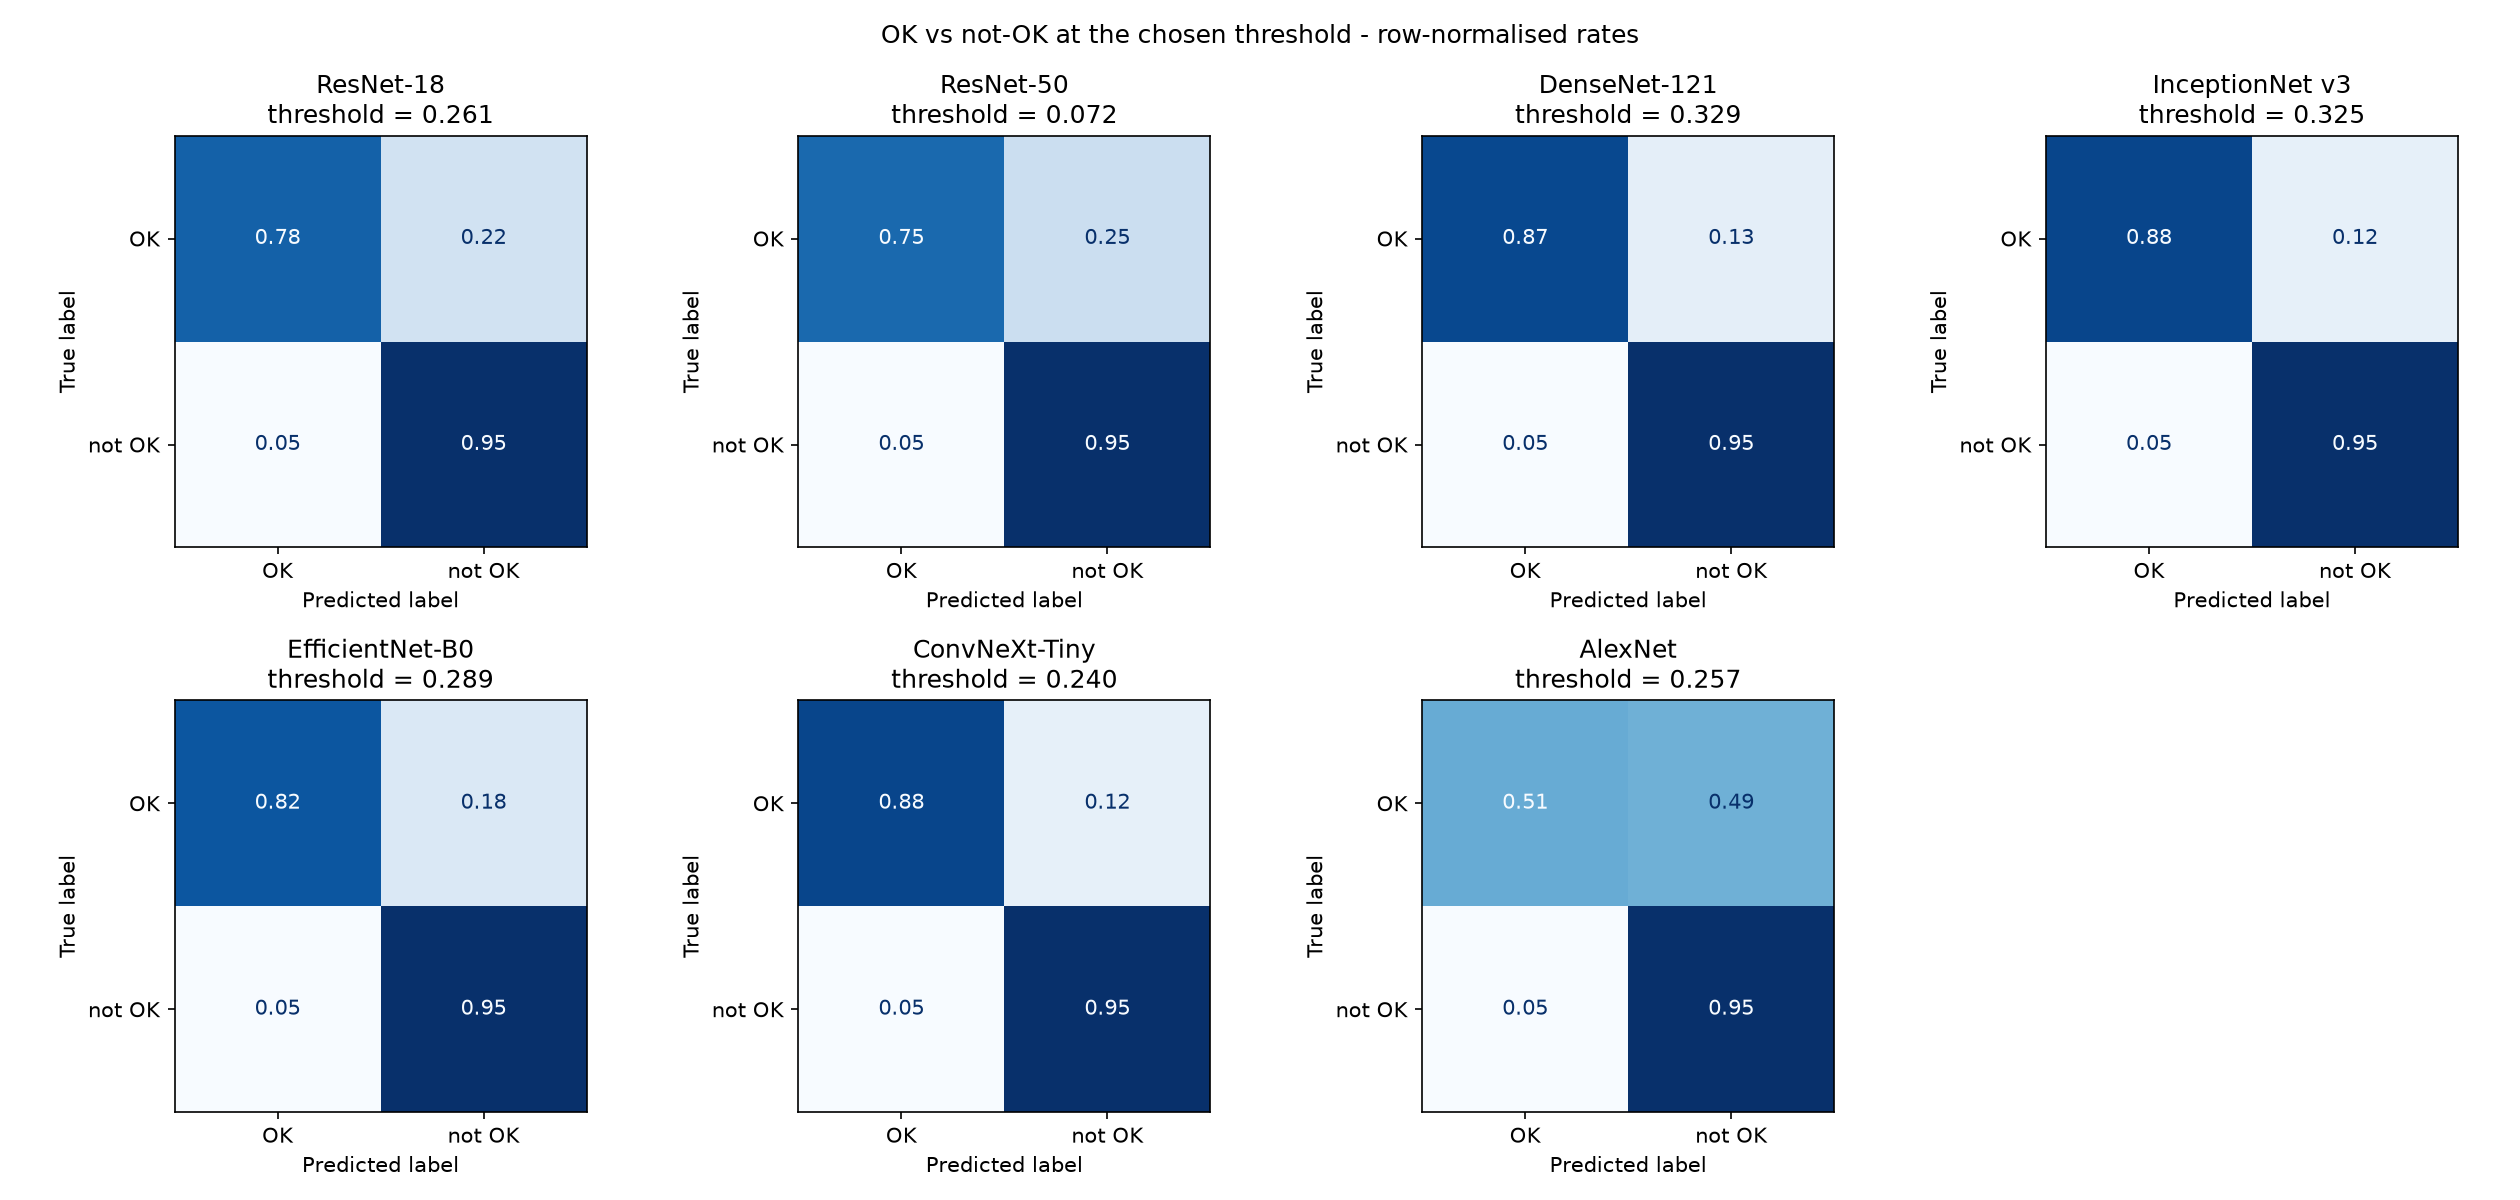
\includegraphics[width=\textwidth]{figures/results/clarifier_stratified_ok_vs_notok_confusion_at_threshold.png}
        \caption{Stratified split}
    \end{subfigure}
    \begin{subfigure}{\textwidth}
        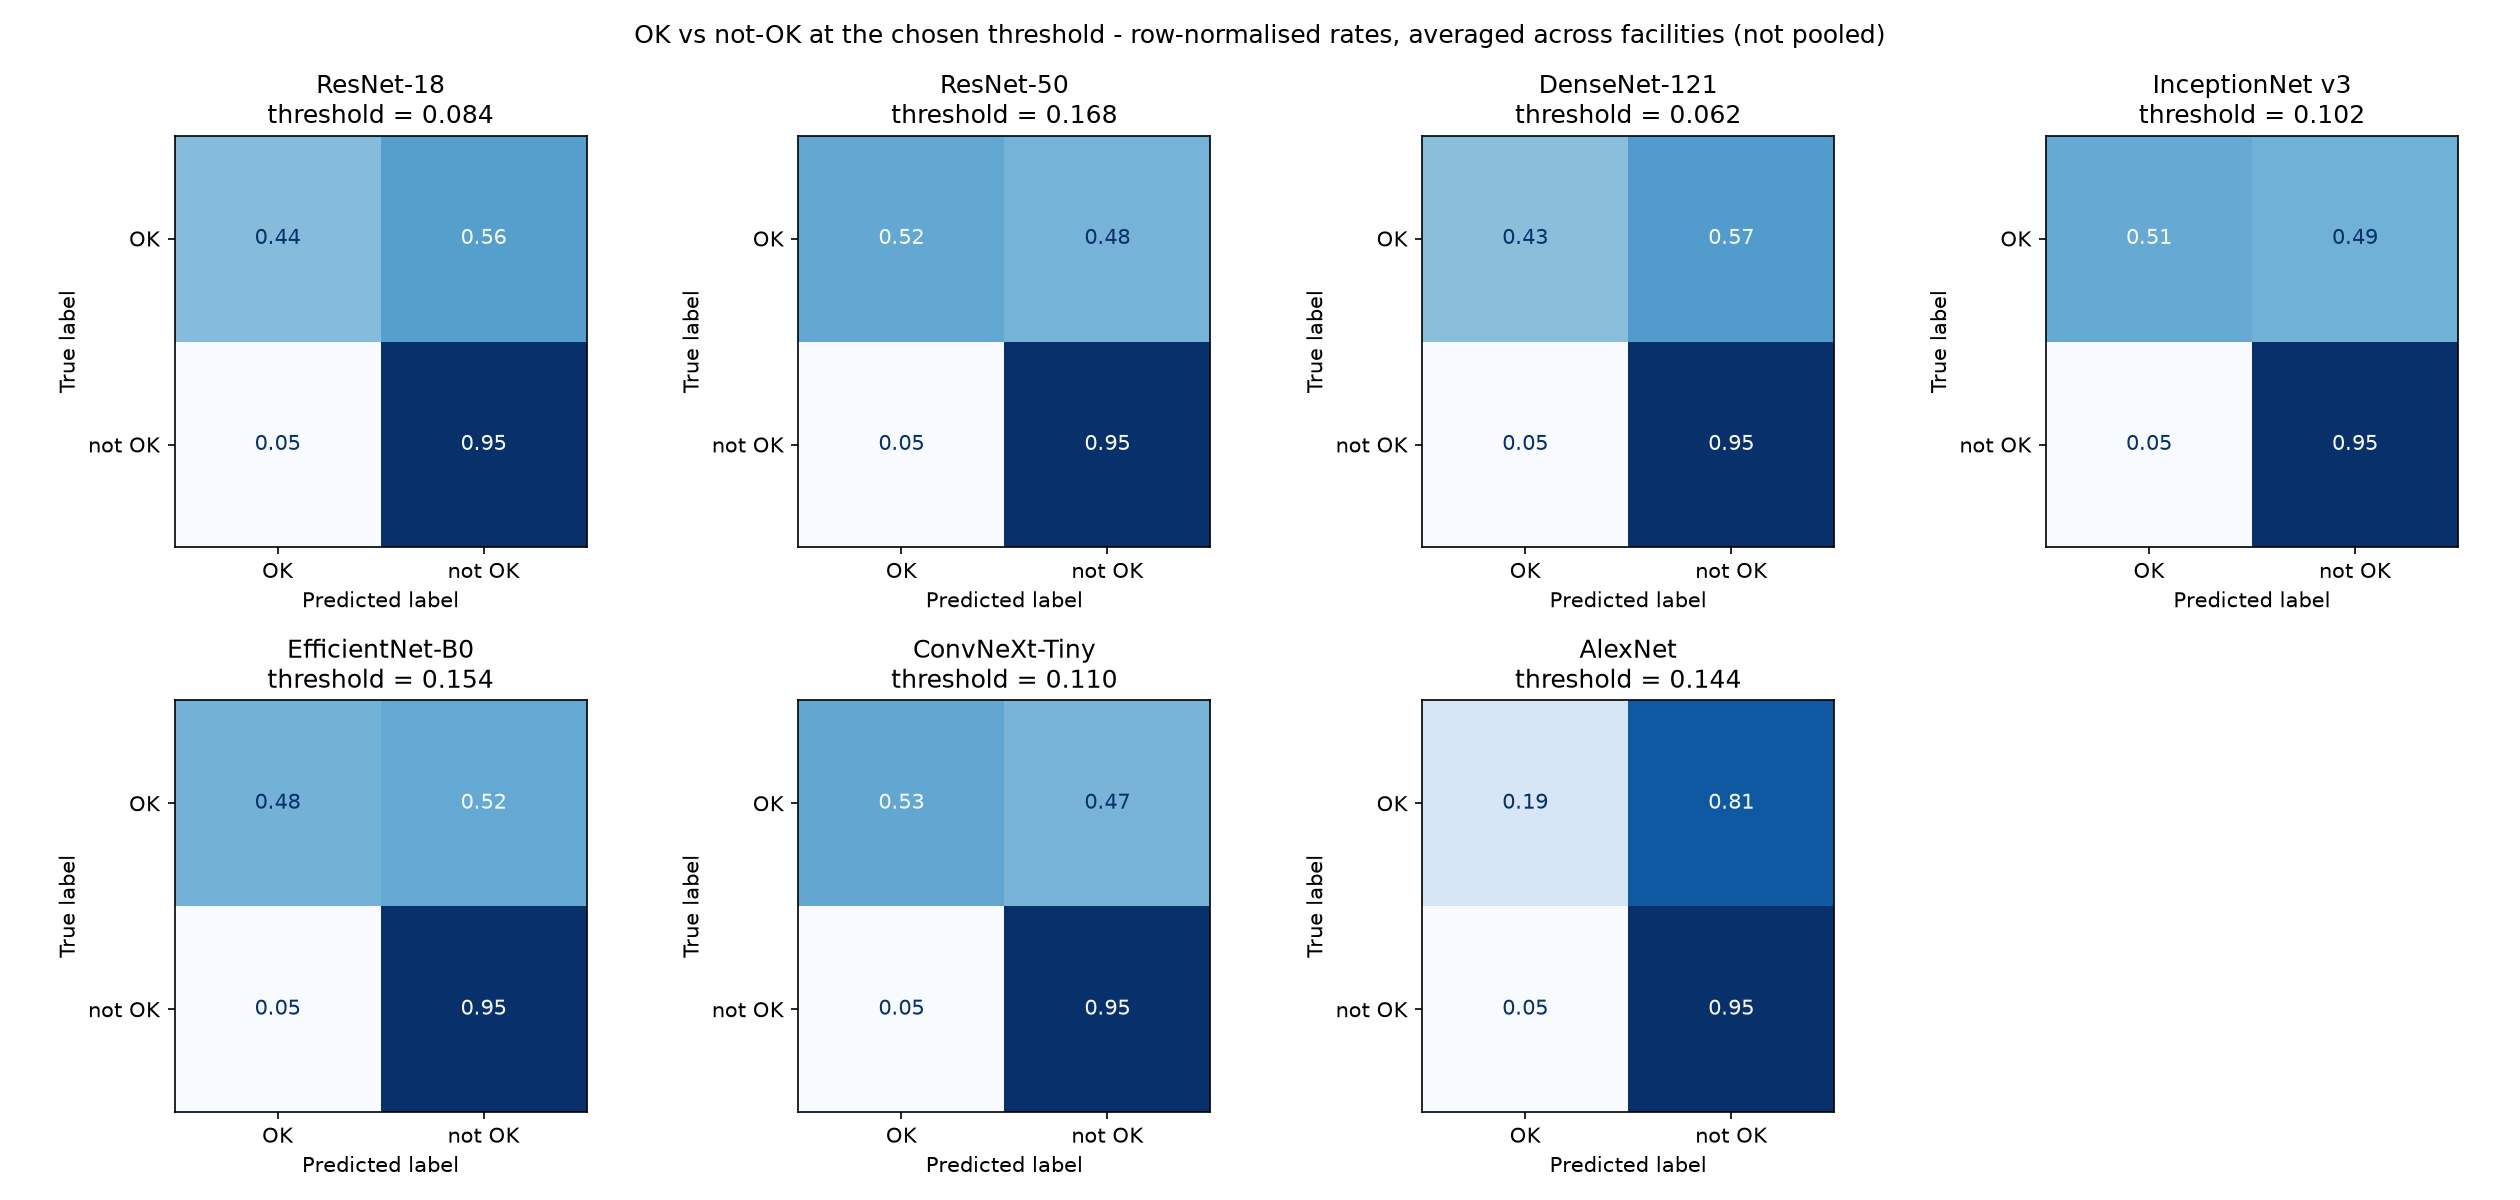
\includegraphics[width=\textwidth]{figures/results/clarifier_lofo_ok_vs_notok_confusion_at_threshold.png}
        \caption{Leave-one-facility-out, averaged across held-out facilities}
    \end{subfigure}
    \caption{Row-normalised binary confusion matrices of the clarifier models at the chosen threshold.}
    \label{fig:res_threshold_clarifier_cm}
\end{figure}

\begin{figure}[htbp]
    \centering
    \begin{subfigure}{\textwidth}
        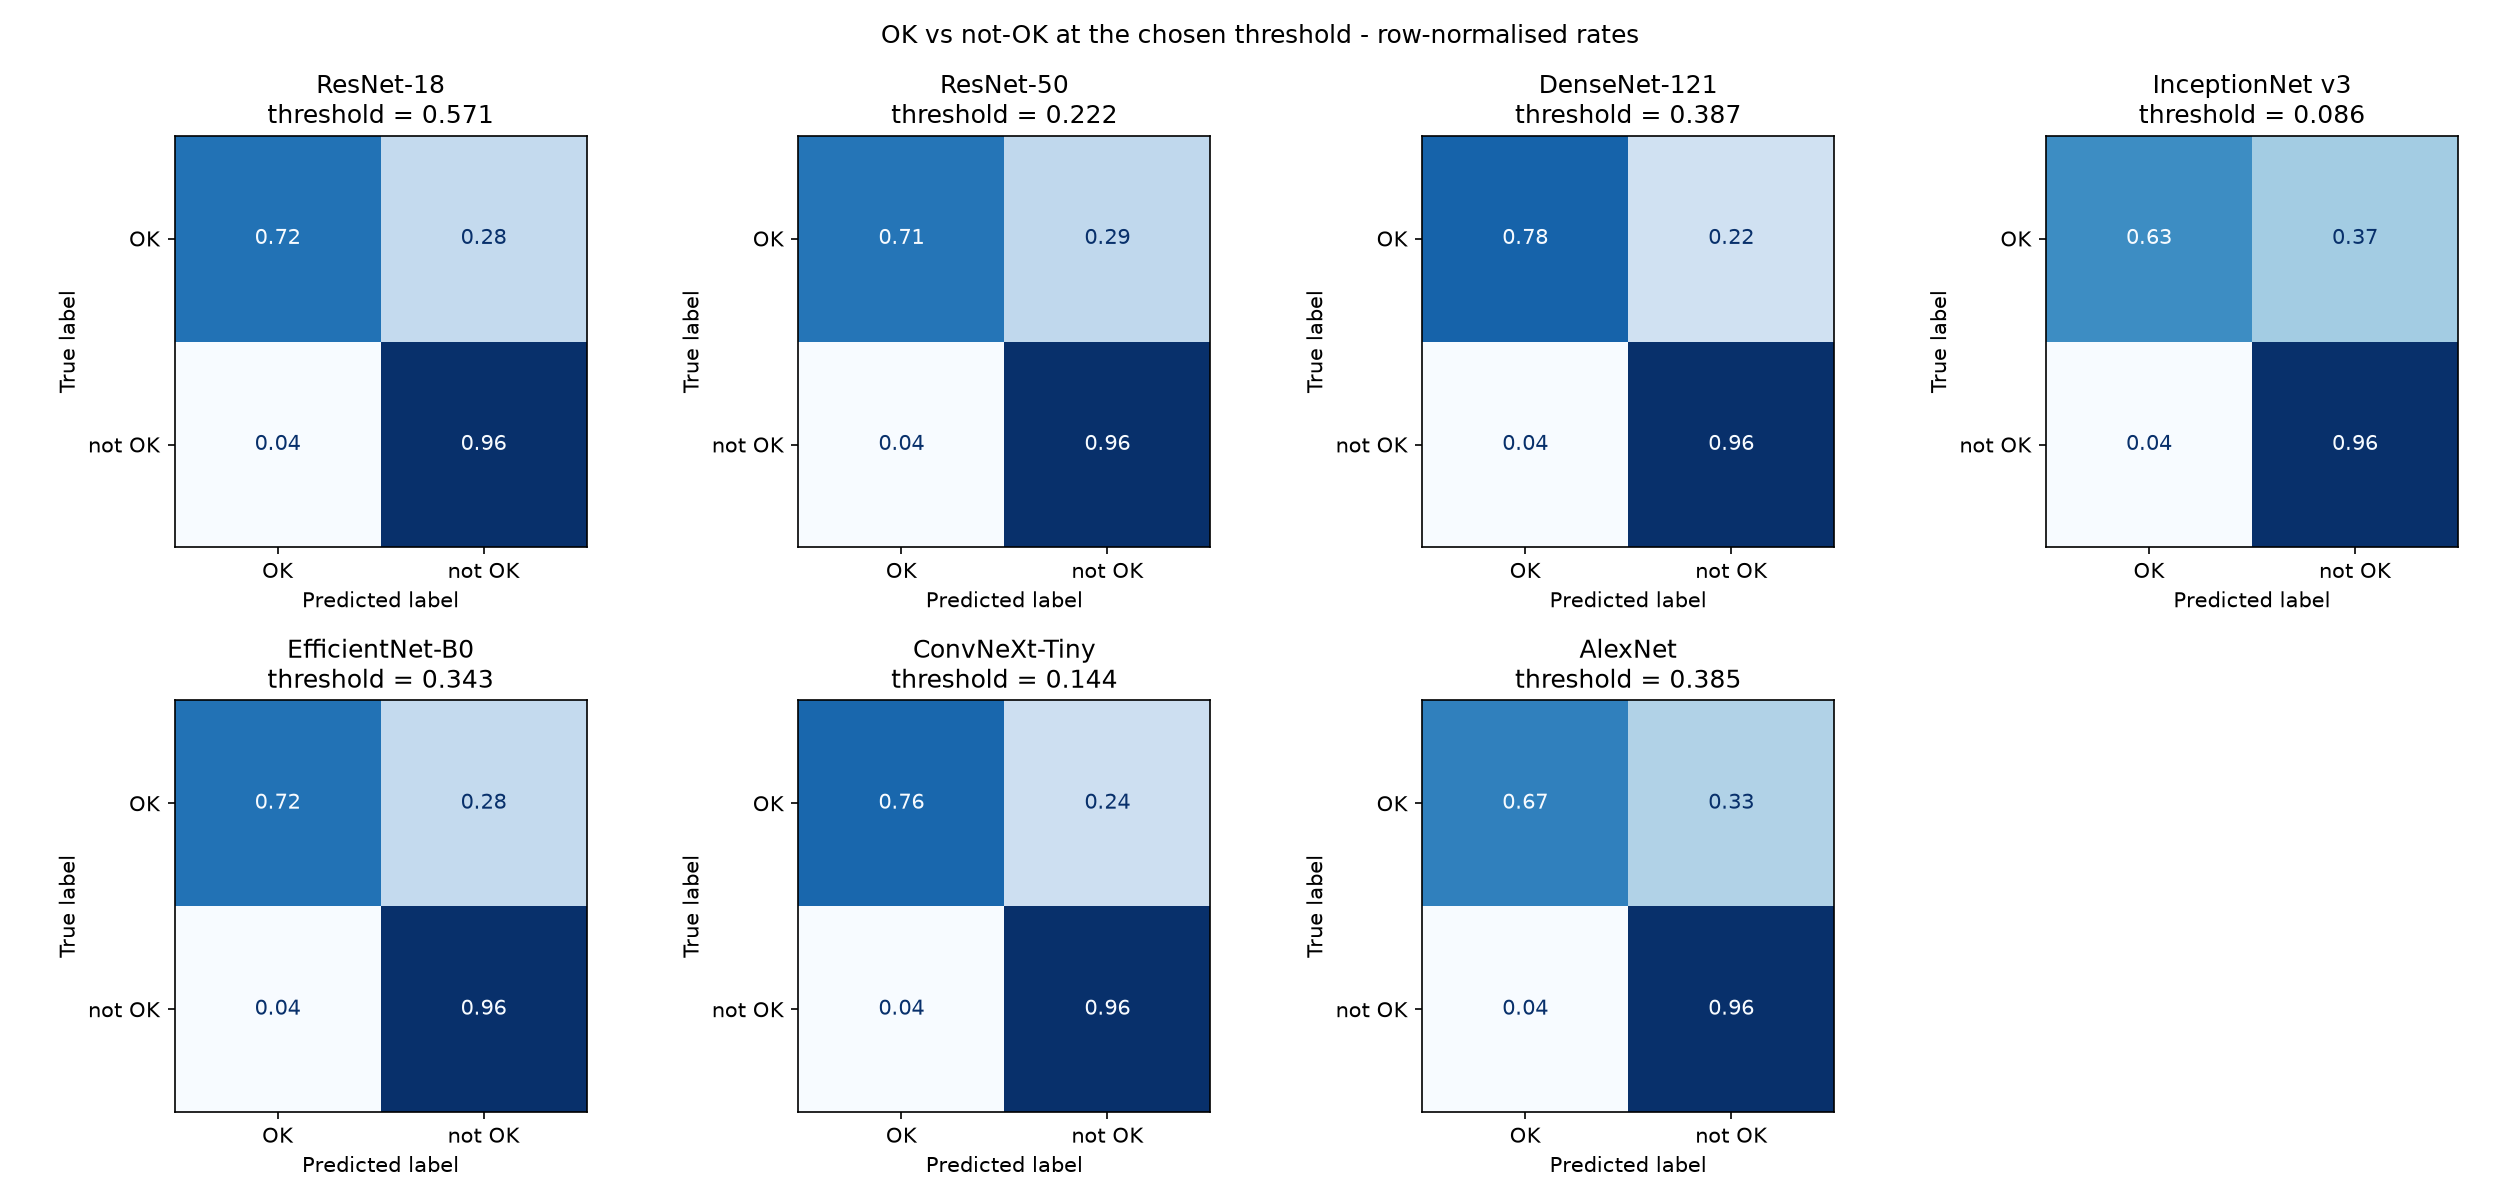
\includegraphics[width=\textwidth]{figures/results/aerobic_zone_stratified_ok_vs_notok_confusion_at_threshold.png}
        \caption{Stratified split}
    \end{subfigure}
    \begin{subfigure}{\textwidth}
        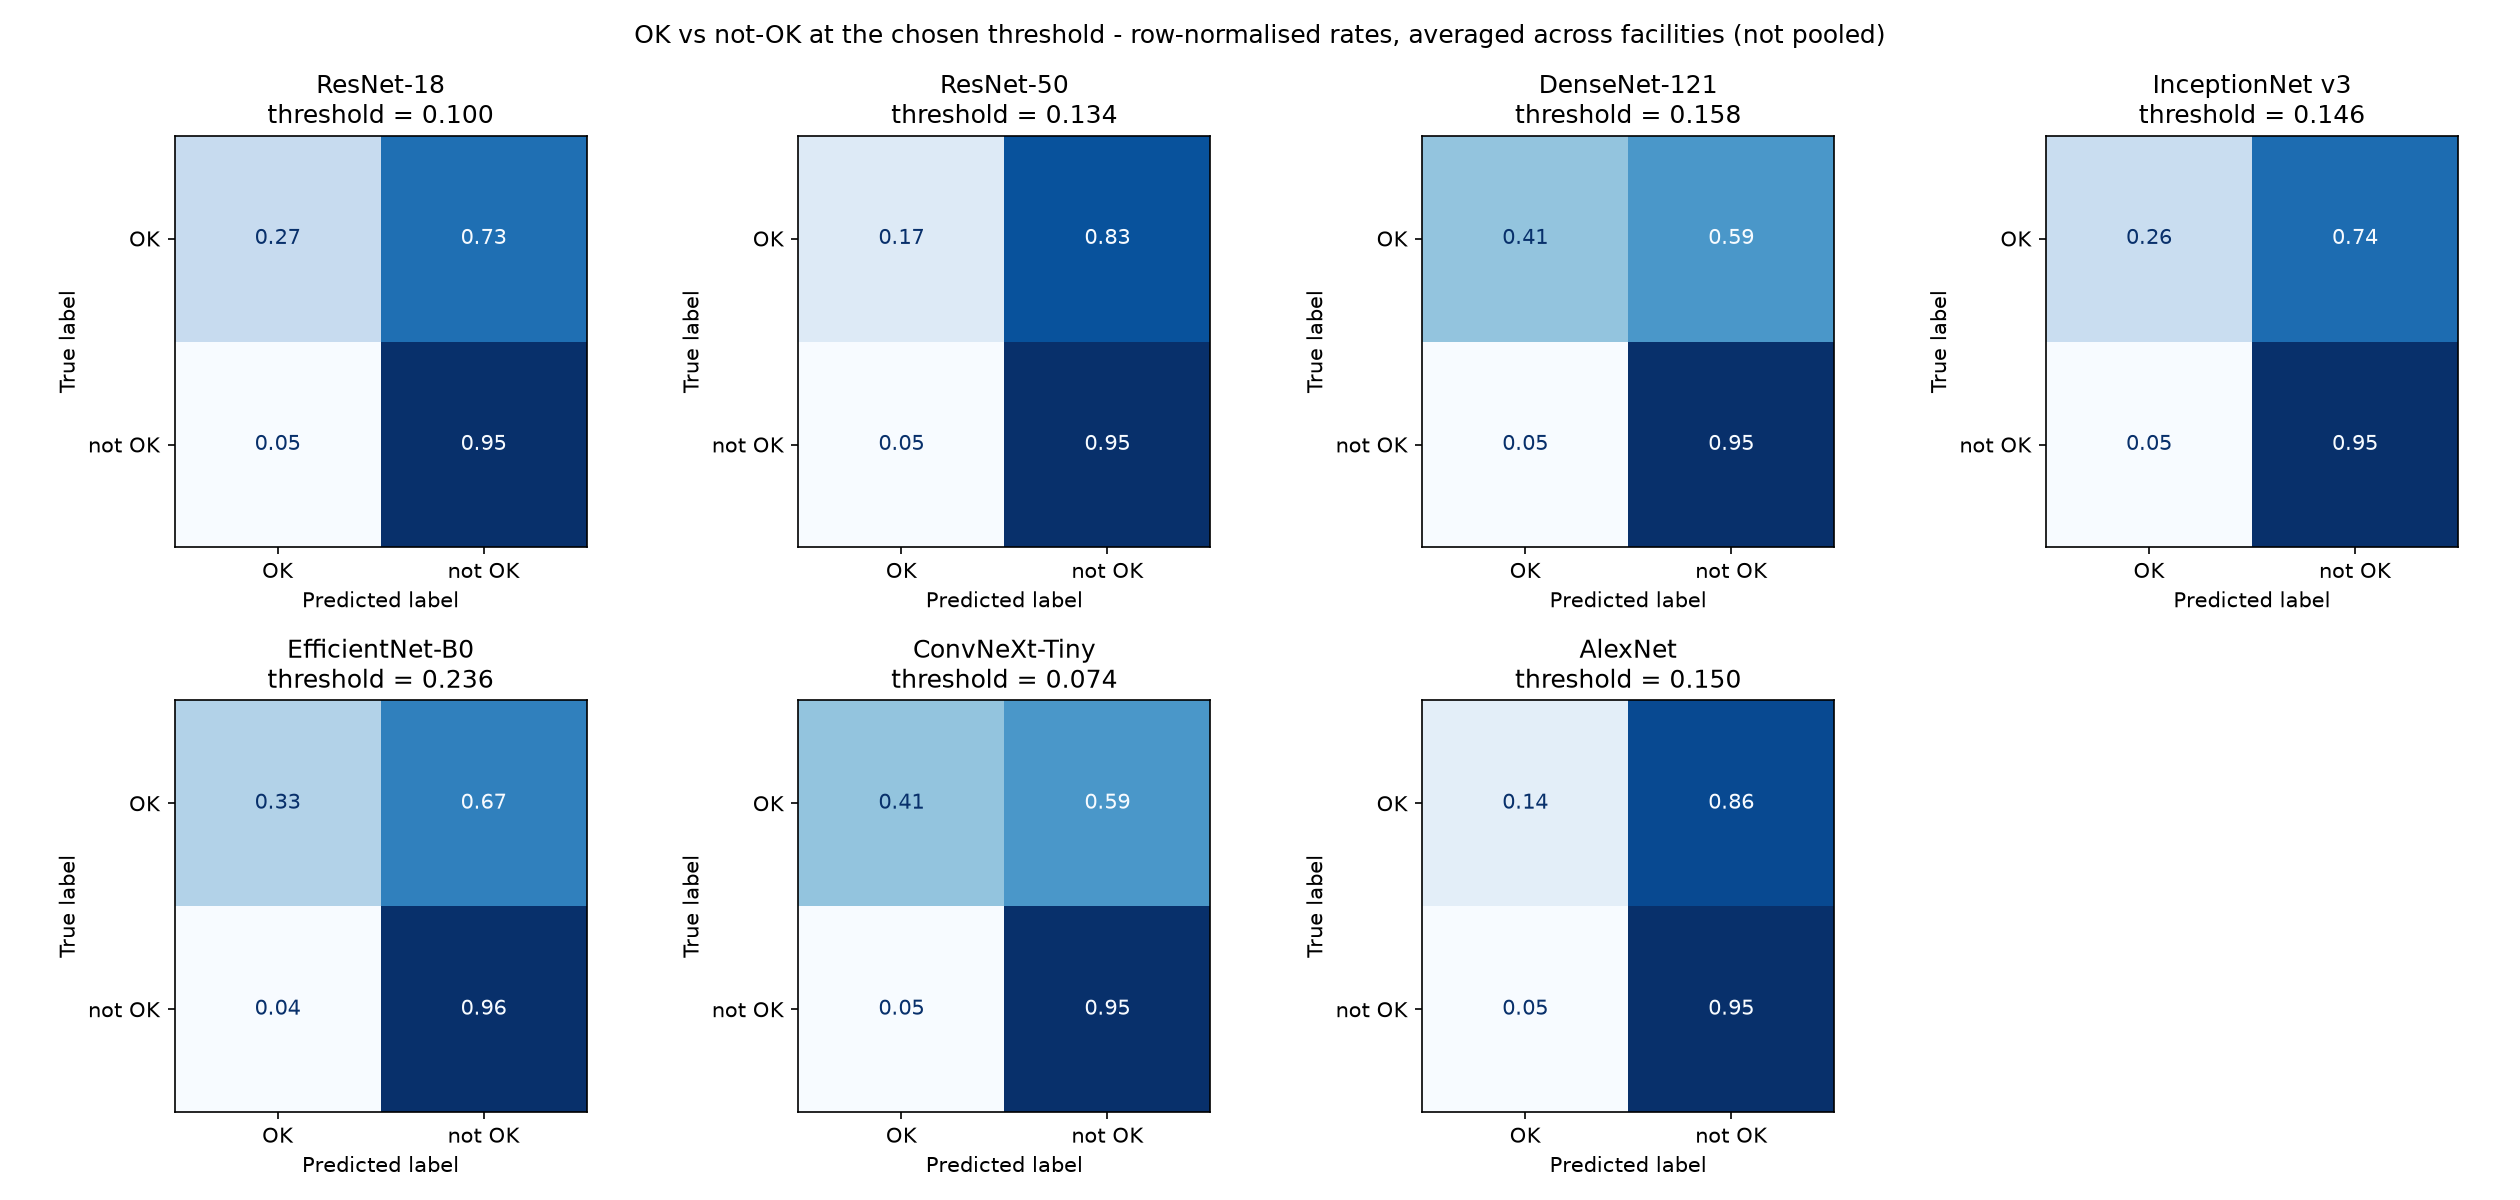
\includegraphics[width=\textwidth]{figures/results/aerobic_zone_lofo_ok_vs_notok_confusion_at_threshold.png}
        \caption{Leave-one-facility-out, averaged across held-out facilities}
    \end{subfigure}
    \caption{Row-normalised binary confusion matrices of the aerobic zone models at the chosen threshold.}
    \label{fig:res_threshold_aerobic_cm}
\end{figure}

\FloatBarrier

\subsection{Threshold Robustness Across Facilities}
\label{sec:results_threshold_robustness}

\begin{table}[htbp]
\centering
\small
\setlength{\tabcolsep}{4pt}
\caption{Recall and specificity of the Not-OK class for each held-out facility at the shared clarifier threshold of Table~\ref{tab:res_threshold}, with the lowest recall and the standard deviation of the recall across facilities.}
\label{tab:res_threshold_robustness_clarifier}
\resizebox{\textwidth}{!}{%
\begin{tabular}{l rrrrr rr}
\toprule
\textbf{Architecture} & \textbf{Atlantis} & \textbf{\makecell[r]{Cape\\Flats}} & \textbf{\makecell[r]{Fisante-\\kraal}} & \textbf{\makecell[r]{Northern\\Works}} & \textbf{Waterval} & \textbf{Min.} & \textbf{Std.} \\
\midrule
\multicolumn{8}{l}{\textit{Recall}} \\
ResNet-18 & 0.909 & 0.995 & 0.901 & 1.000 & 0.949 & 0.901 & 0.046 \\
EfficientNet-B0 & 0.833 & 0.996 & 0.944 & 1.000 & 0.979 & 0.833 & 0.069 \\
DenseNet-121 & 0.894 & 0.997 & 0.859 & 1.000 & 1.000 & 0.859 & 0.068 \\
ResNet-50 & 0.909 & 0.974 & 0.908 & 0.994 & 0.979 & 0.908 & 0.041 \\
ConvNeXt-Tiny & 0.848 & 1.000 & 0.965 & 1.000 & 0.938 & 0.848 & 0.063 \\
Inception-v3 & 0.894 & 0.992 & 0.901 & 0.985 & 0.990 & 0.894 & 0.050 \\
AlexNet & 0.894 & 1.000 & 0.880 & 1.000 & 0.990 & 0.880 & 0.060 \\
\midrule
\multicolumn{8}{l}{\textit{Specificity}} \\
ResNet-18 & 0.841 & 0.080 & 0.491 & 0.086 & 0.708 \\
EfficientNet-B0 & 0.955 & 0.150 & 0.464 & 0.247 & 0.584 \\
DenseNet-121 & 0.818 & 0.108 & 0.855 & 0.086 & 0.292 \\
ResNet-50 & 0.705 & 0.436 & 0.609 & 0.210 & 0.663 \\
ConvNeXt-Tiny & 1.000 & 0.128 & 0.391 & 0.444 & 0.674 \\
Inception-v3 & 0.864 & 0.168 & 0.773 & 0.358 & 0.393 \\
AlexNet & 0.523 & 0.006 & 0.409 & 0.000 & 0.011 \\
\bottomrule
\end{tabular}}
\end{table}

\begin{table}[htbp]
\centering
\small
\caption{Recall and specificity of the Not-OK class for each held-out facility at the shared aerobic zone threshold of Table~\ref{tab:res_threshold}, with the lowest recall and the standard deviation of the recall across facilities.}
\label{tab:res_threshold_robustness_aerobic}
\begin{tabular}{l rrr rr}
\toprule
\textbf{Architecture} & \textbf{Atlantis} & \textbf{Cape Flats} & \textbf{Waterval} & \textbf{Min.} & \textbf{Std.} \\
\midrule
\multicolumn{6}{l}{\textit{Recall}} \\
ResNet-18 & 1.000 & 0.850 & 1.000 & 0.850 & 0.087 \\
EfficientNet-B0 & 0.951 & 0.926 & 0.994 & 0.926 & 0.034 \\
DenseNet-121 & 0.951 & 0.964 & 0.941 & 0.941 & 0.012 \\
ResNet-50 & 1.000 & 0.856 & 1.000 & 0.856 & 0.083 \\
ConvNeXt-Tiny & 1.000 & 0.933 & 0.919 & 0.919 & 0.043 \\
Inception-v3 & 0.951 & 0.967 & 0.931 & 0.931 & 0.018 \\
AlexNet & 1.000 & 0.858 & 1.000 & 0.858 & 0.082 \\
\midrule
\multicolumn{6}{l}{\textit{Specificity}} \\
ResNet-18 & 0.083 & 0.630 & 0.094 \\
EfficientNet-B0 & 0.361 & 0.239 & 0.376 \\
DenseNet-121 & 0.403 & 0.152 & 0.670 \\
ResNet-50 & 0.069 & 0.413 & 0.020 \\
ConvNeXt-Tiny & 0.250 & 0.424 & 0.554 \\
Inception-v3 & 0.500 & 0.109 & 0.168 \\
AlexNet & 0.028 & 0.380 & 0.004 \\
\bottomrule
\end{tabular}
\end{table}

\FloatBarrier


\section{Qualitative Analysis: Grad-CAM}
\label{sec:results_gradcam}

The Grad-CAM method and example selection described in Section~\ref{sec:exp_gradcam} were applied to the architecture with the highest mean macro-averaged F1 score in the leave-one-facility-out experiment for each component: ConvNeXt-Tiny for the clarifiers, tested on Fisantekraal (79.8\% accuracy), and DenseNet-121 for the aerobic zones, tested on Waterval (74.7\% accuracy). The last convolutional layer of these networks is only a $7\times7$ and $3\times7$ grid respectively, so the heatmaps are coarse.

\subsection{Clarifiers}
\label{sec:results_gradcam_clarifiers}

Figure~\ref{fig:gradcam_clarifier} shows the examples for the clarifiers. For the correctly classified \textbf{Dysfunctional}, \textbf{Empty} and \textbf{Scum} clarifiers, the most important region lies on the surface inside the tank. The \textbf{Dysfunctional} heatmap is on the green surface. The \textbf{Empty} heatmap is on the edge of the dark shadow at the top of the tank and on the bright floor below it, which matches the labelling rule that shadows are visible inside an empty tank. The \textbf{Scum} heatmap is on the lower part of the surface, next to the bridge (the arm that spans the tank). The \textbf{Functional} example is the exception: its strongest region is where the bridge meets the rim at the top of the tank, with only weaker regions on the black surface itself.

The ConvNeXt-Tiny heatmaps tend to highlight one or two small regions rather than a larger part of the surface. This is likely related to the global max pooling used in ConvNeXt-Tiny (Section~\ref{sec:exp_architectures}): only the strongest activation of each feature map reaches the classifier head, so the model is trained to respond to the single strongest occurrence of a feature, rather than to how much of the surface it covers.

\begin{figure}[htbp]
    \centering
    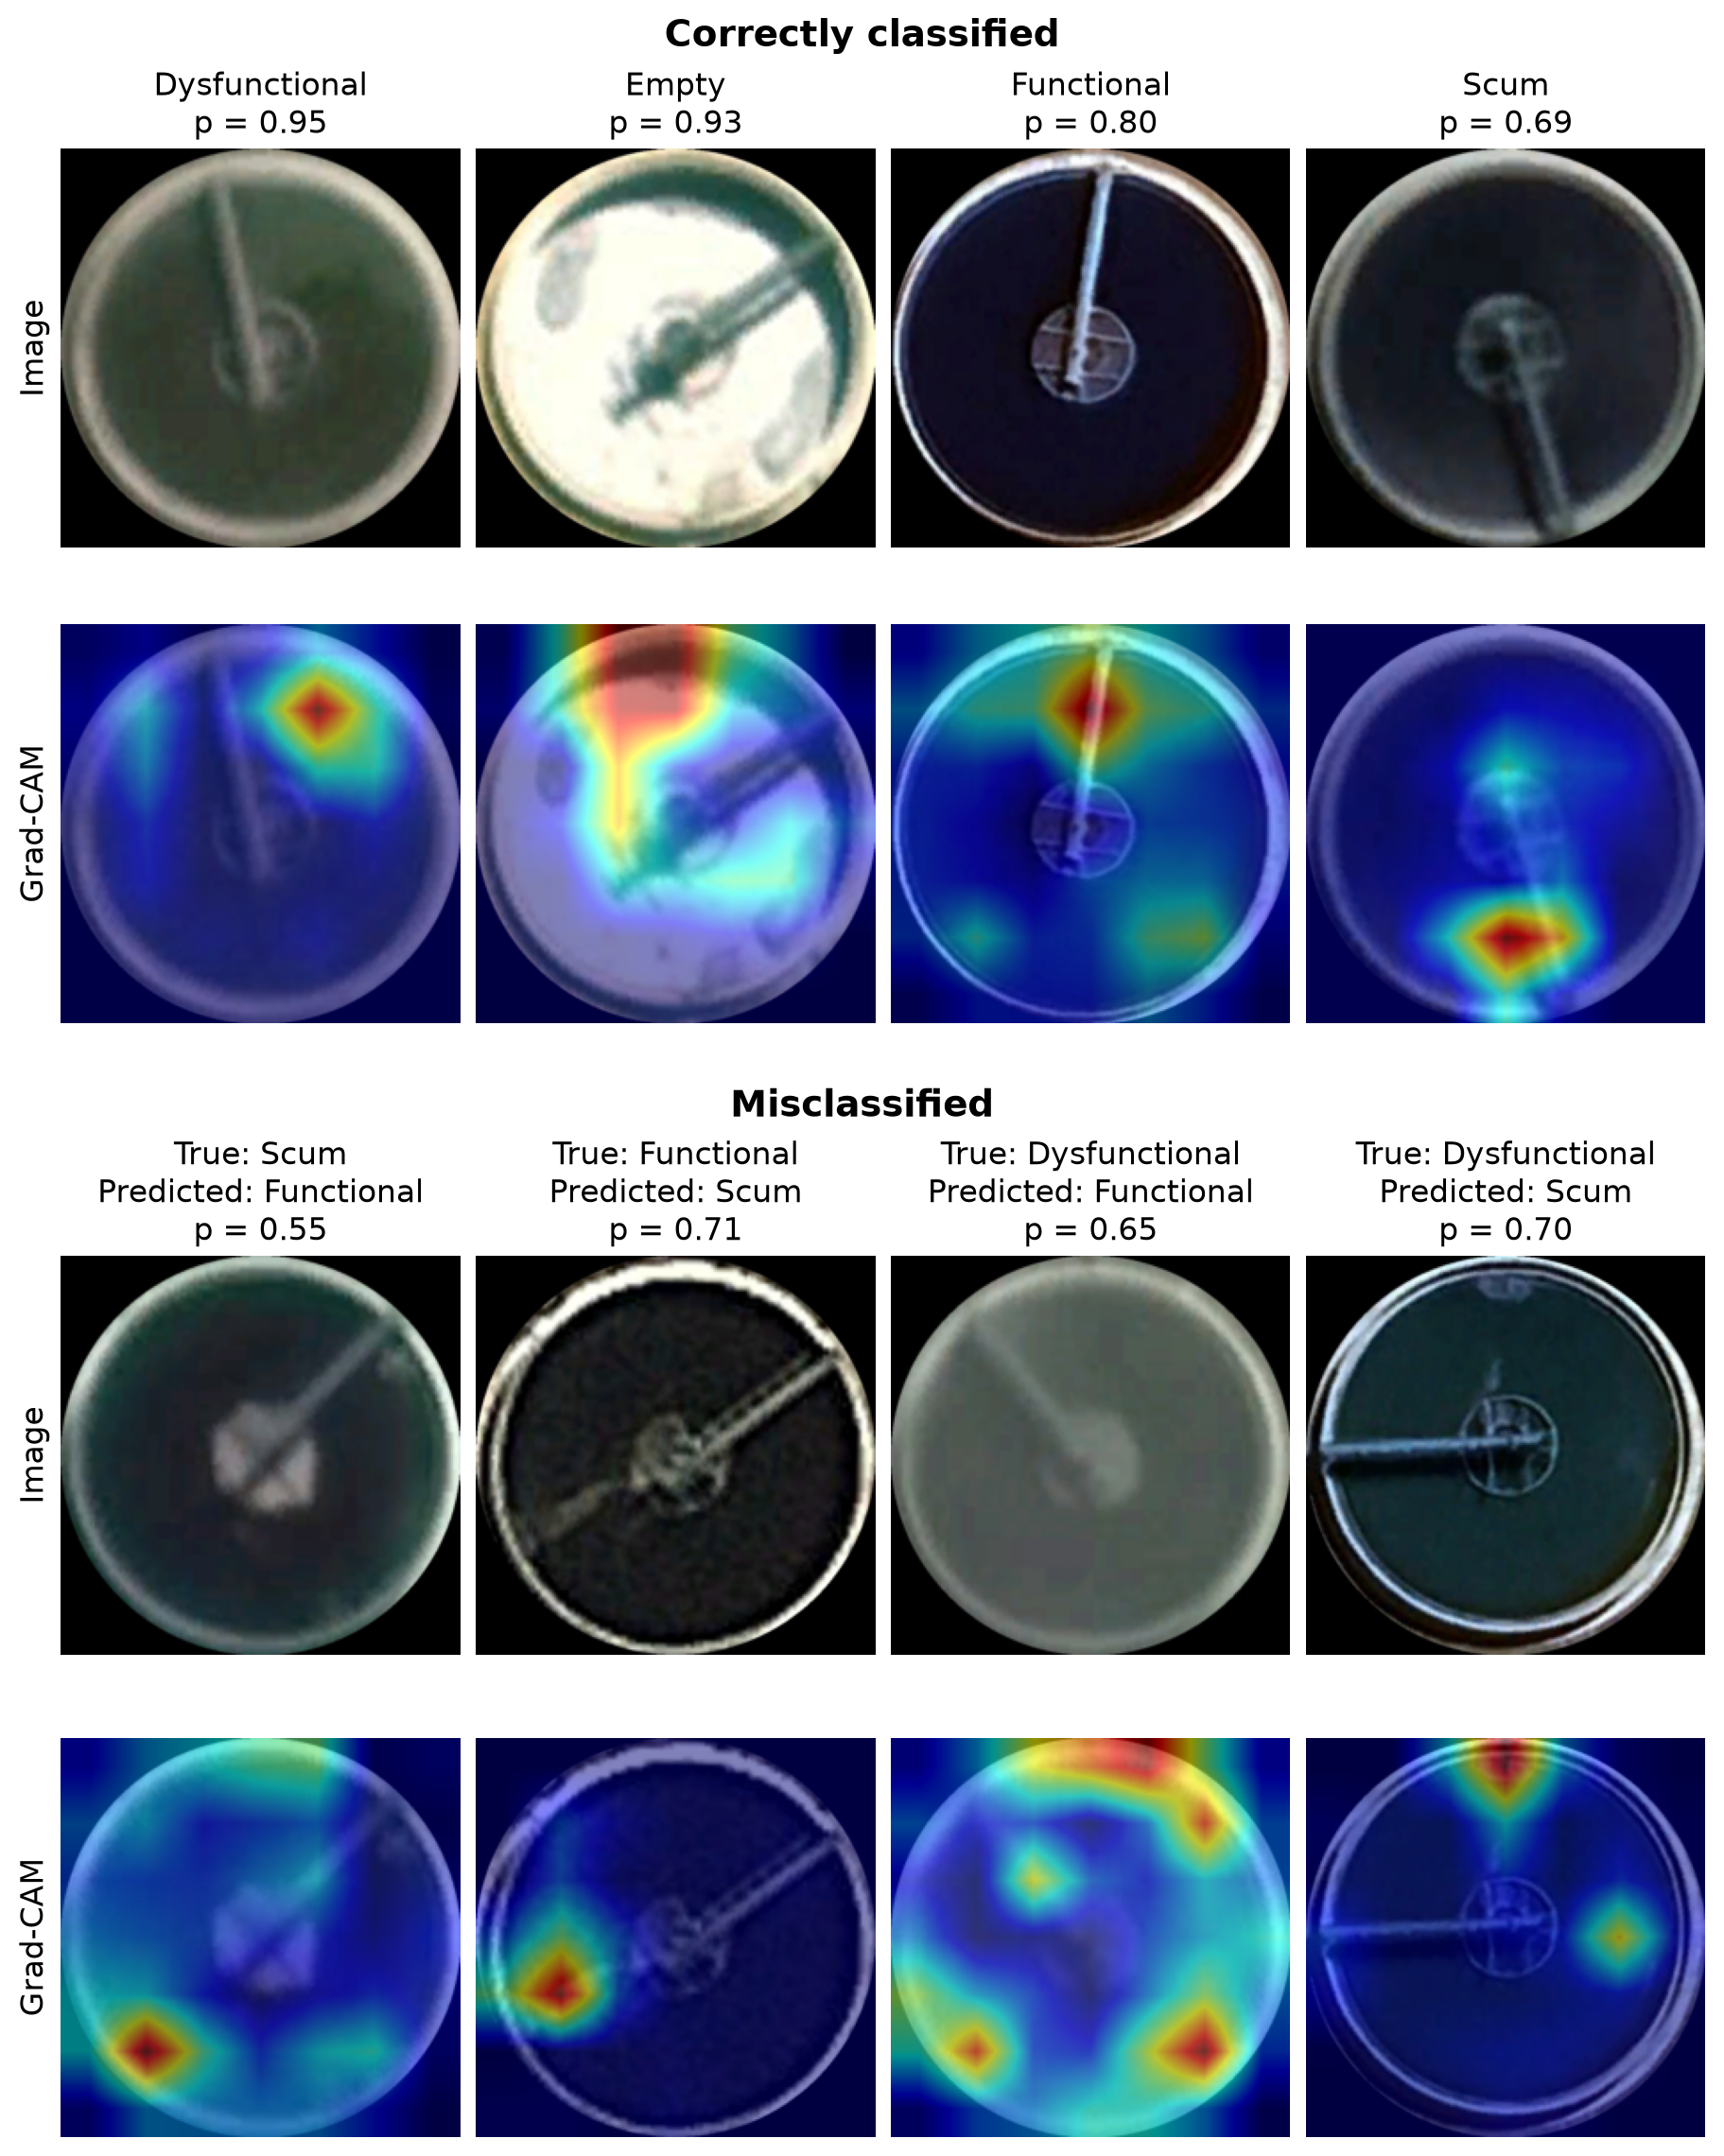
\includegraphics[width=0.85\textwidth]{figures/gradcam_clarifier.png}
    \caption{Grad-CAM heatmaps of the ConvNeXt-Tiny clarifier model, for test images from Fisantekraal, which was held out during training. Top: one correctly classified clarifier per class. Bottom: one clarifier from each of the four most common mistakes. Every heatmap is calculated for the predicted class, and $p$ is the softmax probability of that class. Red regions contributed the most to the prediction.}
    \label{fig:gradcam_clarifier}
\end{figure}

The most common mistake at Fisantekraal is a \textbf{Scum} clarifier classified as \textbf{Functional}, which happened to 26 of the 116 \textbf{Scum} clarifiers. In the example, the light patch around the centre of the tank receives almost no weight, and the prediction is based on the black surface near the edge of the tank. That region on its own does look like a \textbf{Functional} clarifier, but a clarifier only counts as \textbf{Functional} if the whole surface is black. With $p = 0.55$, the model was also unsure of this prediction. The opposite mistake, a \textbf{Functional} clarifier classified as \textbf{Scum}, is shown in the second column. This image is grainy and has a high contrast, so the black surface does not look smooth, and the heatmap lies on the surface at the left edge of the tank. Noise in the image itself could therefore be mistaken for a surface that is not uniformly black.

Only 17 of the Fisantekraal clarifiers are \textbf{Dysfunctional}, but 9 of them were misclassified, and the last two columns show a different problem. In both, most of the weight lies on or next to the concrete rim of the tank rather than on the surface. For the clarifier classified as \textbf{Functional}, part of the heatmap even falls on the black background outside the tank. Neither of these regions says anything about the state of the clarifier. The surface of this clarifier is also a pale grey-green rather than the darker green of the correctly classified \textbf{Dysfunctional} example, so there was little evidence on the surface itself. For the clarifier classified as \textbf{Scum}, the strongest region is on the rim at the top of the tank, with a weaker region on the surface to the right of the centre.

\subsection{Aerobic Zones}
\label{sec:results_gradcam_aerobic}

Figure~\ref{fig:gradcam_aerobic} shows the examples for the aerobic zones. The correctly classified \textbf{Functional} zone is a clear case. The model is certain of its prediction ($p = 1.00$), and the heatmap covers the centre of the zone, where the leopard print pattern is visible. This is the feature an operator would look for, which suggests that the model has learned to recognise it. The correctly classified \textbf{Dysfunctional} and \textbf{Suboptimal} zones are much less certain, with $p = 0.49$ and $p = 0.43$, which is only a little above the $0.33$ of a random guess between three classes. For the \textbf{Dysfunctional} zone, the heatmap covers the smooth surface at the left end of the zone. For the \textbf{Suboptimal} zone, it covers a band in the right half of the zone, where the surface is slightly darker and uneven.

\begin{figure}[htbp]
    \centering
    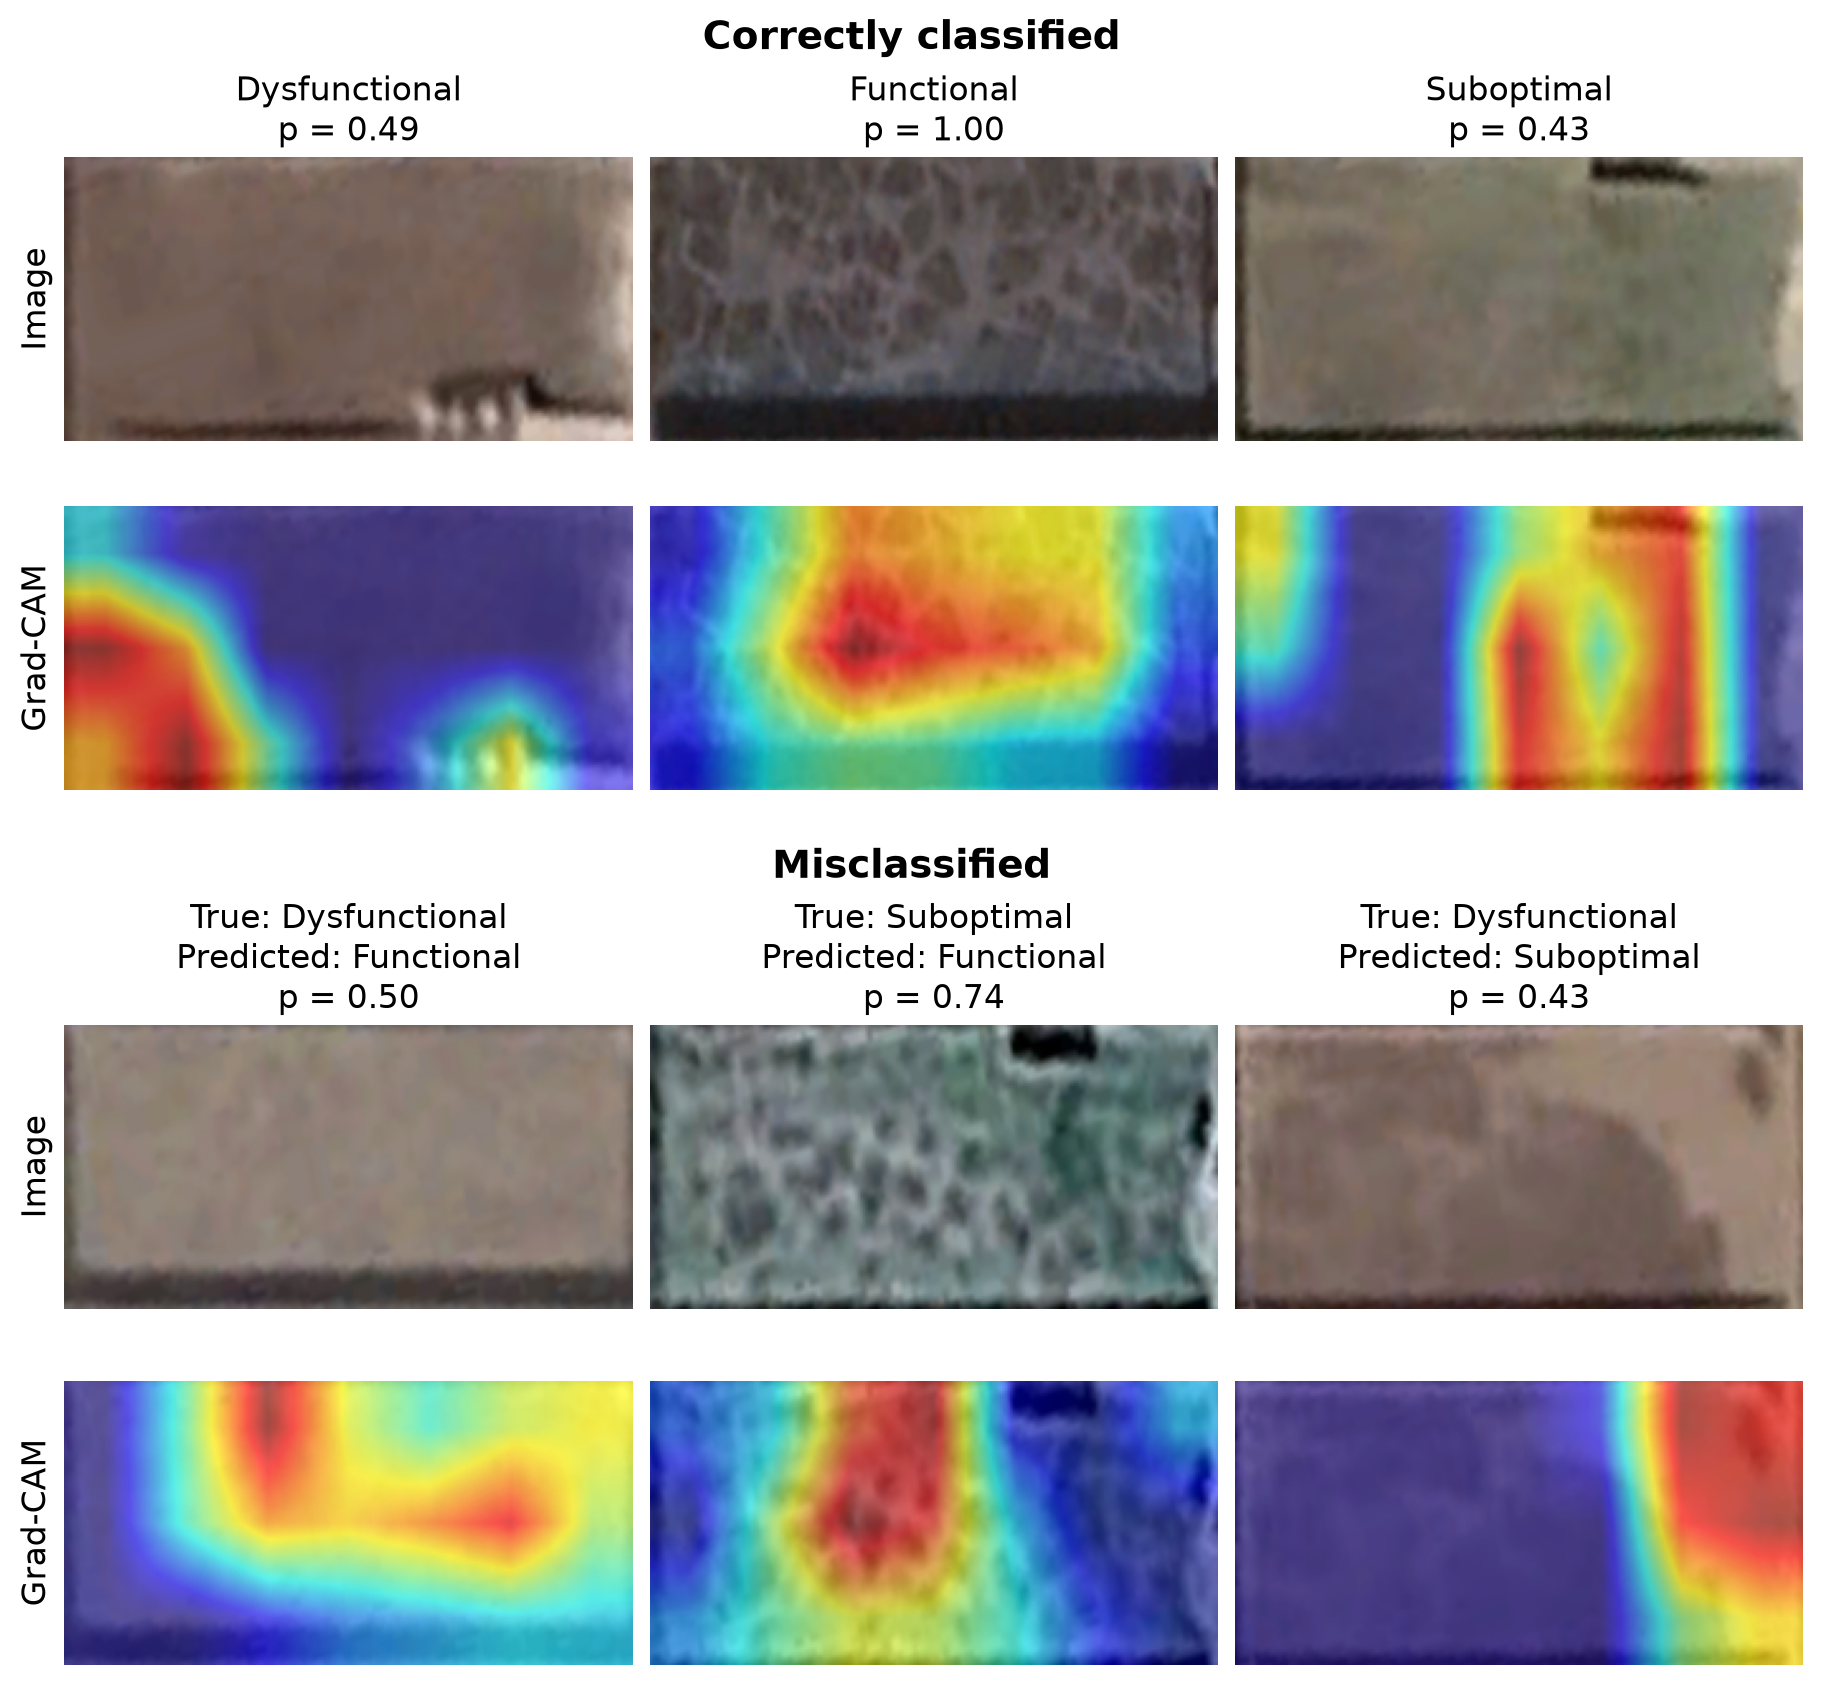
\includegraphics[width=0.9\textwidth]{figures/gradcam_aerobic_zone.png}
    \caption{Grad-CAM heatmaps of the DenseNet-121 aerobic zone model, for test images from Waterval, which was held out during training. Top: one correctly classified aerobic zone per class. Bottom: one aerobic zone from each of the three most common mistakes. Every heatmap is calculated for the predicted class, and $p$ is the softmax probability of that class. Red regions contributed the most to the prediction.}
    \label{fig:gradcam_aerobic}
\end{figure}

Both of the most common mistakes at Waterval are zones classified as \textbf{Functional}: 100 of the 229 \textbf{Dysfunctional} zones and 74 of the 92 \textbf{Suboptimal} zones. The \textbf{Suboptimal} example in the second column shows part of the reason. The left and centre of the zone show a clear leopard print pattern, while the right third is smooth. The heatmap lies on the patterned centre, and the smooth part receives almost no weight. According to the labelling rules in Chapter~\ref{chap:systemmethods}, a zone is \textbf{Suboptimal} once a third or more of its surface shows no leopard print, so the class depends on how much of the surface is patterned. The model found the pattern where it exists, but did not take into account how much of the surface it covers. This zone is also close to the boundary between the two classes, and since only the clarifier labels were reviewed (Chapter~\ref{chap:systemmethods}), some of these mistakes may partly be caused by the aerobic zone labels themselves.

The \textbf{Dysfunctional} zone classified as \textbf{Functional}, in the first column, has a smooth surface with no visible pattern, and its heatmap is spread over a large part of the zone rather than on one specific feature. With $p = 0.50$, the model was unsure, and there is no clear feature in the image that it could have mistaken for the leopard print. For the \textbf{Dysfunctional} zone classified as \textbf{Suboptimal}, the heatmap is on a darker patch at the right end of the zone, which does not look like the aeration pattern either.

\subsection{Summary of Observations}
\label{sec:results_gradcam_summary}

When the models were confident and correct, they mostly looked at the features the labels are based on. The mistakes show two problems. For \textbf{Scum} and \textbf{Suboptimal}, which depend on how much of the surface shows a feature, the models based their prediction on the strongest region and gave little weight to the rest. When the surface gave little evidence either way, the heatmaps spread out or moved to the rim of the tank, and the confidence was low. These are only a few examples, but they are consistent with the most common mistakes at both facilities.


\section{Summary of Findings}
\label{sec:results_summary}
